\documentclass[10pt,a4paper]{article}
\usepackage[utf8]{inputenc}
\usepackage[english,russian]{babel}
\usepackage[OT1]{fontenc}
\usepackage{amsmath}
\usepackage{amsfonts}
\usepackage{amssymb}
\usepackage{graphicx}
\usepackage{float}
\usepackage{wrapfig}
\usepackage{caption}
\DeclareCaptionLabelSeparator{dot}{. }
\captionsetup{justification=centering,labelsep=dot}
\graphicspath{{pictures/}}
\DeclareGraphicsExtensions{.pdf,.png,.jpg,.eps}
\begin{document}

\part{Основы}

 \textbf{\Large3 Фильтры Гаусса}\\
 
 \textbf{3.1 Введение}\\
 
 В этой главе описывается важное семейство рекурсивных методов оценки состояния под общим названием «фильтры Гаусса». Исторически, гауссовы фильтры образуют класс самых ранних управляемых реализаций байесовских фильтров для непрерывных пространств. Несмотря на имеющиеся недостатки, они также являются наиболее популярным семейством методов на сегодняшний день.
 
 Все гауссовы методы используют основную идею представления оценок в виде многомерных нормальных распределений. Мы уже сталкивались с определением многомерного нормального распределения в Выражении (2.4), но, для удобства, приведём его ещё раз\\
 
 (3.1)$$p(x)=det(2\pi\varSigma)^{-\frac{1}{2}}exp\left\lbrace-\frac{1}{2}(x-\mu)^T\varSigma^{-1}(x-\mu)\right\rbrace $$
 Эта плотность по переменной $x$ характеризуется двумя наборами параметров: математическим ожиданием $\mu$ и ковариационной матрицей $\varSigma$. Математическое ожидание $\mu$ - это вектор, имеющий ту же размерность, что и вектор состояний $x$. Ковариационная матрица представляет собой квадратную симметричную неотрицательно определённую матрицу, размерность которой равна квадрату размерности вектора состояний $x$. В силу этого число элементов в ковариационной матрице квадратично зависит от количества элементов в векторе состояний.
 
 Стремление представить апостериорные вероятности в виде нормального распределения имеет важные последствия. Важнее всего то, что гауссовы распределения одномодальны – они имеют единственный максимум. Такая апостериорнная вероятность характерна для многих проблем отслеживания состояния в робототехнике, она концентрируется вокруг реального состояния с небольшим диапазоном неопределённости. Нормальные апостериорные распределения плохо подходят для глобальных задач оценки, где имеется множество отдельных гипотез, каждая из которых образует собственную моду в апостериорном распределении.
 
 ПАРАМЕТРИЗАЦИЯ МОМЕНТОВ
 
 Задание параметров нормального распределения в виде математического ожидания и ковариационной матрицы называется параметризацией в виде моментов (moments parameterization), поскольку математическое ожидание и ковариация – это моменты первого и второго порядка вероятностного распределения (для нормальных распределений все остальные моменты равны нулю).\\
 КАНОНИЧЕСКАЯ ПАРАМЕТРИЗАЦИЯ\\
 В данной главе мы также обсудим другой способ задания параметров, называемый канонической параметризацией, или, иногда, обычной параметризацией. Оба вида параметризации, каноническая и в виде моментов, функционально эквиваленты и образуют взаимно однозначные выражения, которые можно трансформировать друг в друга, но имеют несколько различные вычислительные характеристики. Как мы увидим, канонический и натуральный способ задания параметров лучше всего воспринимать как взаимодополняющие: то, что выглядит вычислительно лёгким в одном виде параметризации, используется в другом, и наоборот.
 В этой главе вводятся два основных алгоритма фильтра Гаусса.\\
 
 • В подразделе 3.2 описан фильтр Калмана, реализующий байесовский фильтр с заданием параметров в виде моментов для решения ограниченного класса задач с линейной динамикой и функциями измерения.\\
 
 • В подразделе 3.3 описан обобщенный фильтр Калмана, алгоритм которого приспособлен для решения нелинейных задач.
 
 • В подразделе 3.4 приводится описание другого нелинейного фильтра Калмана, известного как unscented Kalman filter.
  
 • В подразделе 3.5 описан информационный фильтр, дополняющий фильтр Калмана, используя каноническую  параметризацию гауссовых функций.\\
 
 \textbf{3.2 Фильтр Калмана}\\
  
 \textbf{3.2.1 Линейные гауссовы системы}\\
 Возможно, наиболее известный метод использования байесовских фильтров – это фильтр Калмана или ФК (KF). Фильтр Калмана был открыт Свирлингом (Swerling, 1958) и Калманом (Kalman, 1960) как способ фильтрации и прогнозирования для \textit{линейных гауссовых систем}, которые определение которых сейчас будет приведено. Фильтр Калмана выполняет вычисление оценок только для непрерывных состояний и неприменим для дискретных или гибридных пространств состояний.\\
 АПОСТЕРИОРНАЯ ГАУССОВА ВЕРОЯТНОСТЬ
  
 Фильтр Калмана отображает оценки в виде моментов: для момента времени $t$, оценка представлена математическим ожиданием $\mu_t$ и ковариационной матрицей $\varSigma_t$. Апостериорные вероятности представлены \textit{функциями Гаусса} если, вдобавок к марковским допущениям для байесовских фильтров, соблюдаются 3 следующих свойства:\\
 
 1. Аргументы переходной вероятности состояния $p(x_t | u_t,x_{t-1})$ должны быть линейными функциями с добавочным гауссовским шумом. Это выражается следующим равенством:\\
 
 (3.2)$$x_t=A_{t} x_{t-1} +B_{t}u_{t}+\varepsilon_t$$
 Здесь $x_t$ и $x_{t-1}$ - векторы состояния, а $u_t$ – вектор управления в момент времени $t$. В данной записи оба вектора имеют вид вертикальной матрицы
 
 (3.3)
 \begin{minipage}{0.3\textwidth}
 	\begin{equation*}
 	x_t=
 	\left(\begin{array}{c}
 	x_{1,t}\\
 	x_{2,t}\\
 	\vdots\\
 	x_{n,t}\\
 	\end{array}\right)
 	\end{equation*}
 \end{minipage}
 \begin{minipage}{0.3\textwidth}
 	\begin{equation*}
  	\mbox {и} \hspace{10mm} u_t=
 	\left(\begin{array}{c}
 	u_{1,t}\\
 	u_{2,t}\\
 	\vdots\\
 	u_{m,t}\\
 	\end{array}\right)
 	\end{equation*}
 \end{minipage}
{}\\

 $A_t$ – это квадратная матрица размера $n\times n$, где $n$ - размерность вектора состояний $x_t$. Прямоугольная матрица $B_t$ имеет размер $n\times m$, где $m$ –размерность вектора управления $u_t$. После перемножения векторов состояния и управления с матрицами $A_t$ и $B_t$, соответственно,  функции перехода состояний приобретает \textit{линейные} аргументы. Таким образом, в фильтрах Калмана достигается линейная динамика системы.\\
  
 Случайная переменная $\varepsilon_t$ в (3.2) представляет собой случайный гауссовый вектор, предназначенный для моделирования неопределённости, привносимой переходом состояний. Он имеет ту же размерность, что и вектор состояний, его математическое ожидание равно нулю, а ковариацию обозначим через $R_t$. Вероятность перехода состояний вида (3.2) называется \textit{линейным гауссианом}, отражая факт линейности аргументов с добавлением гауссового шума. Технически, в (3.2) возможно прибавить и дополнительную константу, но в излагаемом материале она никакой роли не играет, поэтому её можно опустить.\\
 
 Выражение (3.2) определяет переходную вероятность состояния $p(x_t | u_t, x_{t-1})$. Эта вероятность получается после вставки уравнения (3.2) в определение многомерного нормального распределения (3.1). Математическое ожидание апостериорного состояния задано в виде $A_{t}x_{t-1}+B_{t}u_t$, а ковариация - $R_t$:\\
 
 (3.4)
 \begin{multline*}
 $$p(x_t|u_t,x_{t-1})=det(2\pi R_t)^{-\frac{1}{2}}\\
 exp\left\lbrace -\frac{1}{2}(x_t-A_{t}x_{t-1}-B_{t}u_t)^T R_t^{-1}(x_t-A_{t}x_{t-1}-B_{t}u_t)\right\rbrace$$ 
 \end{multline*}
 \begin{table}[h]
 \begin{center}
 \begin{tabular}{|l|}
 \hline
 {}\\
 1: \hspace{3mm} Algorithm Kalman\_filter $(\mu_{t-1},\varSigma_{t-1},u_t,z_t):$ \\
 {}\\
 2: \hspace{7mm} 
 $\bar{\mu}_t=A_t \mu_{t-1}+B_t u_t$\\
 3: \hspace{7mm} $\bar{\varSigma}_t=A_t \varSigma_{t-1}A_t^T+R_t$\\
 {}\\
 4: \hspace{7mm} $K_t=\bar{\varSigma}_t C_t^T(C_t \bar{\varSigma}_t C_t^T+Q_t)^{-1}$\\
 5: \hspace{7mm} $\mu_t=\bar{\mu}_t+K_t(z_t-C_t \bar{\mu}_t)$\\
 6: \hspace{7mm}  $\varSigma_t=(I-K_t C_t)\bar{\varSigma}_t$\\
 7: \hspace{7mm}
 \textit{return} $\mu_t,\varSigma_t$\\
 {}\\
 \hline
 \end{tabular}
 \caption{(Таблица 3.1 Алгоритм фильтра Калмана для линейных гауссовых переходов состояний и измерений. )}
 \end{center}
 \end{table}\\

2. Вероятность измерения $p(z_t | x_t)$ также должна иметь \textit{линейные аргументы} с добавленным гауссовым шумом:\\

(3.5) $$z_t=C_t x_t+\delta_t$$

Здесь $C_t$ - это матрица размера $k\times n$, где $k$ – размерность вектора измерений $z_t$. Вектором $\delta_t$ описывается шум измерений. Распределение $\delta_t$ представляет собой многомерную нормальную функцию с нулевым математическим ожиданием и ковариацией $Q_t$. Отсюда, вероятность измерения задаётся следующим многомерным нормальным распределением:\\

(3.6)$$p(z_t|x_t)=det(2\pi Q_t)^{-\frac{1}{2}}exp\left\lbrace -\frac{1}{2}(z_t-C_t x_t)^T Q_t^{-1}(z_t-C_t x_t)\right\rbrace$$

3. И, наконец, первоначальная оценка $bel(x_0)$ должна быть нормально распределена. Обозначим математическое ожидание этой величины $\mu_0$, а ковариацию - $\varSigma_0$:

(3.7)$$bel(x_0)=p(x_0)=det(2\pi \varSigma_0)^{-\frac{1}{2}}exp\left\lbrace-{\frac{1}{2}}(x_0-\mu_0)^T\varSigma_0^{-1}(x_0-\mu_0)\right\rbrace$$

Этих трёх условий достаточно, чтобы гарантировать, что апостериорное распределение $bel(x_t)$ для любого момента времени $t$ всегда будет гауссовой функций. Доказательство этого нетривиального утверждения можно найти ниже, в математическом выводе для фильтра Калмана (Подраздел 3.2.4).\\

\textbf{3.2.2 Алгоритм фильтра Калмана}\\

Алгоритм фильтра Калмана приводится в Таблице 3.1. Фильтры Калмана выражают оценку $bel(x_t)$ в момент времени $t$ через математическое ожидание $\mu_t$ и ковариацию $\varSigma_t$. На вход фильтр Калмана принимается оценка в момент времени $t-1$, выраженная через $\mu_{t-1}$ и $\varSigma_{t-1}$. Для обновления этих параметров требуются также управляющее воздействие $u_t$ и измерение $z_t$. Выводом является оценка в момент времени $t$, выраженная через $\mu_t$ и $\varSigma_t$.

В строках 2 и 3 вычисляются прогнозируемые значения $\bar{\mu}$ и $\bar{\varSigma}$, выражая оценку $\overline{bel}(x_t)$ для следующего такта времени, но до учёта измерений $z_t$. Эта оценка получается путём учёта управляющего воздействия $u_t$. Математическое ожидание обновляется, используя детерминированную версию функции перехода состояния (3.2), с математическим ожиданием $\mu_{t-1}$, заменённую для состояния $x_{t-1}$. Обновление ковариации учитывает факт зависимости новых состояний от предыдущих, отражённый
линейной матрицей $A_t$. Эта матрица дважды умножается на значение ковариации, поскольку ковариация выражена квадратичной матрицей.

В строках с 4 по 6 происходит последовательное преобразование оценки $\overline{bel}(x_t)$  в требуемую оценку $bel(x_t)$ с учётом измерения $z_t$.\\
УСИЛЕНИЕ ФИЛЬТРА КАЛМАНА\\
Переменная $K_t$, вычисленная в строке 4, называется \textit{усилением фильтра Калмана}. Она определяет степень, до которой измерение учитывается в новой оценке состояния. Как именно это происходит - будет разъяснено в Подразделе 3.2.4. Строка 5 управляет математическим ожиданием, меняя его пропорционально усилению фильтра Калмана $K_t$, отклонению текущего измерения, $z_t$, а также прогнозируемому измерению (3.5).\\
КОРРЕКЦИЯ\\
Ключевой концепцией здесь является \textit{коррекция}, которая представляет собой разницу между реальным измерением $z_t$ и ожидаемым измерением $C_t \bar{\mu}_t$ в строке 5. Наконец, в строке 6 вычисляется новая ковариационная матрица апостериорной оценки, учитывающая добавочную информацию, полученную в результате измерения.

Фильтр Калмана довольно эффективен в вычислительном смысле. Для лучших, на сегодняшний день, алгоритмов сложность инверсии матрицы размером $d\times d$ составляет, приблизительно, $O(d^{2.4})$. Каждая итерация фильтра Калмана, как уже было сказано, ограничена снизу сложностью (приблизительно) $O(k^{2.4})$, где $k$ – размерность вектора измерений $z_t$. Эта, (снова, приблизительно), кубическая степень сложности получается в силу инверсии матрицы в строке 4. Даже для некоторых случаев с разреженным обновлением, описанных в будущих главах, она составляет, по крайней мере $O(n^2)$, где $n$ – размерность пространства состояний, из-за перемножения в строке 6 (матрица $K_t C_t$ может быть разреженной). Для многих реализаций (например, задачи построения карт, обсуждаемой в более поздних главах) пространство измерений имеет намного меньшую размерность по сравнению с пространством состояний, и такт обновления, в основном, состоит из операций сложности $O(n^2)$.\\


\begin{figure}[h]
	\center{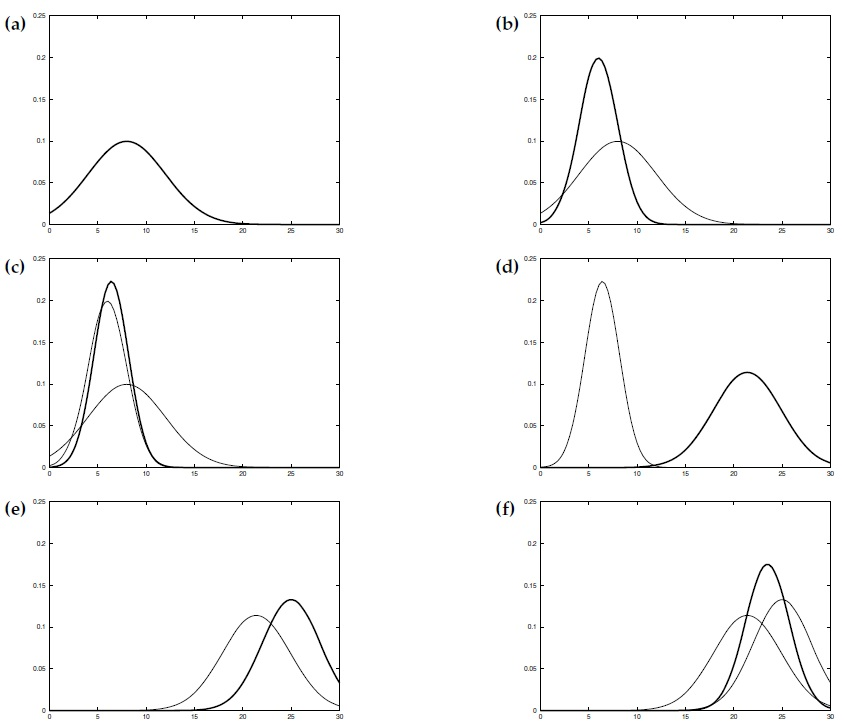
\includegraphics[width=1\linewidth]{32orig}}
	\caption{ (  Рис. 3.2 Иллюстрация работы фильтров Калмана: (a) первоначальная оценка, (b) измерение (выделено жирным) с соответствующей неопределённостью, (c) оценка после учёта измерения алгоритмом фильтра Калмана, (d) оценка после движения вправо (которое вносит дополнительную неопределённость), (e) новое измерение с соответствующей неопределённостью, и (f) результирующая оценка.)}
	\label{fig:32orig}
\end{figure}

\textbf{3.2.3 Иллюстрация}\\

На Рис. 3.2 показан алгоритм фильтра Калмана для простейшего одномерного сценария локализации. Допустим, на каждой диаграмме Рис. 3.2 робот двигается вдоль горизонтальной оси. Пусть априорная оценка местоположения робота задана нормальным распределением, показанным на Рис. 3.2a. Робот запрашивает данные своего местоположения с датчиков (например, системы GPS), и возвращает результат измерения с центром на пике выделенной жирным  функции Гаусса на Рис. 3.2b. Выделенный жирным график гауссовой функции раскрывает представление измерения: пик обозначает прогнозируемое согласно показаниям датчиков значение, а ширина (дисперсия) связана с неопределённостью измерения. Результат комбинирования априорной оценки и измерения, выполненный в строках с 4 по 6 алгоритма фильтра Калмана в Таблице 3.1, приведён в виде  жирного графика гауссианы на Рис. 3.2c. Значение математического ожидания этой оценки лежит между двух первичных пиков, а радиус неопределённости - меньше, чем у обоих предыдущих гауссовых функций. Факт того, что остаточная неопределённость меньше, чем у исходных нормальных распределений, может показаться контринтуитивным, но он является общей характеристикой интеграции информации в калмановских фильтрах.

Далее, допустим, робот движется направо. Степень неопределённости возрастает в силу стохастической природы перехода состояния. Строки 2 и 3 калмановского фильтра дают гауссову кривую, показанную жирным на Рис. 3.2d. Эта кривая сдвинута на величину перемещения робота, и, в силу только что озвученных причин, шире. Робот получает данные второго измерения, показанные жирной чертой на графике гауссовой функции на Рис. 3.2e, которое, затем, даёт апостериорную оценку, показанную на Рис. 3.2f.

Как показано на примере, в алгоритме фильтра Калмана последовательно чередуются такты обновления измерений (строки 5-7), в которых данные датчиков интегрируются в текущую оценку, и прогнозирования (или, иначе, такты обновления управления), которые модифицируют оценку в соответствии с действием. Такт обновления уменьшает, а такт прогнозирования – увеличивает неопределённость оценки робота.\\
 
\textbf{3.2.4 Математический вывод фильтра Калмана}\\

В этом разделе выполняется вывод алгоритмов фильтрации Калмана из Таблицы 3.1. Его можно смело пропускать при первом прочтении, поскольку он приводится из соображений полноты изложения.

Во-первых, вывод KF, по большей части, это упражнение по манипулированию квадратичными выражениями. Экспоненты складываются, например, при перемножении двух гауссовых функций. Поскольку обе первичные экспоненты квадратичные, результирующая сумма тоже. После этого останется только представить результат в форме, допускающей определение целевых параметров.\\
 
\textbf{Часть 1: Прогнозирование}\\

Вывод начинается со строк 2 и 3 алгоритма, в которых оценка $\overline{bel}(x_t)$ вычисляется на основе оценки, полученной на предыдущем шаге, $bel(x_{t-1})$. В строках 2 и 3 выполняется такт обновления,  описанный в Выражении (2.41), и приведённого здесь для удобства читателя:\\

(3.8)$$\overline{bel}(x_t)=\int \underbrace{p(x_t|x_{t-1},u_t)}_{\sim N(x_t;A_t x_{t-1}+B_t u_t,R_t)}\underbrace{bel(x_{t-1})}_{\sim N(x_{t-1};\mu_{t-1},\varSigma_{t-1})}dx_{t-1}
$$

Оценка $bel(x_{t-1})$ представлена математическим ожиданием $\mu_{t-1}$ и ковариацией $\varSigma_{t-1}$. Переходная вероятность $p(x_t | x_{t-1}, u_t)$ была дана в (3.4) в виде нормального распределения по $x_t$ с математическим ожиданием $A_t x_{t-1}+B_t u_t$ и ковариацией $R_t$. Как сейчас будет продемонстрировано, результат (3.8) тоже представляет собой гауссову функцию с математическим ожиданием $\bar{\mu}_t$ и ковариацией $\bar{\varSigma}_t$, как указано в Таблице 3.1.

Начнём с записи (3.8) в виде гауссовой функции:\\

(3.9)
\begin{multline*}
$$\overline{bel}(x_t)\\=\eta \int \exp\left\lbrace -\frac{1}{2}(x_t-A_t x_{t-1}-B_t u_t)^T R_t^{-1}(x_t-A_t x_{t-1}-B_t u_t)\right\rbrace\\ \exp\left\lbrace -\frac{1}{2}(x_{t-1}-\mu_{t-1})^T \varSigma_{t-1}^{-1}(x_{t-1}-\mu_{t-1})\right\rbrace dx_{t-1}$$ 
\end{multline*}

После сокращения, получим\\

(3.10)
$$\overline{bel}(x_t)=\eta \int \exp\left\lbrace -L_t\right\rbrace dx_{t-1}$$ 

где\\

(3.11)
\begin{multline*}
$$L_t=\frac{1}{2}(x_t-A_t x_{t-1}-B_t u_t)^T R_t^{-1}(x_t-A_t x_{t-1}-B_t u_t)\\ +\frac{1}{2}(x_{t-1}-\mu_{t-1})^T \varSigma_{t-1}^{-1}(x_{t-1}-\mu_{t-1})$$ \end{multline*}

Заметим, что $L_t$ квадратично как для $x_{t-1}$, так и для $x_t$.

Выражение (3.10) содержит интеграл, решение которого требует переопределения членов на интервале интегрирования. Способ разложения, поначалу, кажется контринтуитивным. В частности,  выполним разложение $L_t$ на две функции, $L_t(x_{t-1}, x_t)$ и $L_t(x_t)$:\\

(3.12)
$$L_t=L_t(x_{t-1},x_t)+L_t(x_t)$$

Это разложение будет просто результатом перегруппировки членов в $L_t$ и главной его целью  должно стать разделение переменных в $L_t$ на два множества, из которых только одно будет зависеть от переменной $x_{t-1}$. Другое, $L_t(x_t)$, от $x_{t-1}$ зависеть не будет. В результате, второй набор переменных можно вынести из-под интеграла по переменной $x_{t-1}$.

Это показано следующим преобразованием:\\

(3.13)
 
\begin{multline*}
$$\overline{bel}(x_t)=\eta\int\exp\left\lbrace -L_t\right\rbrace dx_{t-1}\\ 
=\eta\int\exp\left\lbrace-L_t(x_{t-1},x_t)-L_t(x_t)\right\rbrace dx_{t-1}\\ =\eta  \exp\left\lbrace -L_t(x_t)\right\rbrace\int\exp\left\lbrace -L_t(x_{t-1},x_t)\right\rbrace dx_{t-1}$$ 
\end{multline*}

Конечно, существует множество способов разложить $L_t$ на два множества, удовлетворяющие этому критерию. Ключевой мыслью будет выбор $L_t(x_{t-1},x_t)$ таким образом, чтобы значение интеграла в (3.13) не зависело от  $x_t$. Если нам удастся определить такую функцию $L_t(x_{t-1} ,x_t)$, весь интеграл по $L_t(x_{t-1},x_t)$ в задаче определения распределения по $x_t$, станет просто константой. Константы обычно учитываются в нормализующей постоянной $\eta$, поэтому в нашем разложении возможно включить константу в $\eta$ (её значение будет отличаться от константы $\eta$, приводимой выше):\\

(3.14)
$$\overline{bel}(x_t)=\eta \exp\left\lbrace -L_t(x_t)\right\rbrace $$

Таким образом, разложение делает возможным исключение интеграла из оценки (3.10). Результатом является нормализованная экспонента квадратичной функции, представляющая собой нормальное распределение.

Давайте выполним это разложение. Мы ищем функцию $L_t(x_{t-1},x_t)$, квадратичную для $x_{t-1}$. (Эта функция будет также зависеть от $x_t$, но сейчас это неважно.) Для определения коэффициентов квадратичной функции вычислим первые две производные $L_t$:\\

(3.15)
$$\frac{\partial L_t}{\partial x_{t-1}}=-A_t^T R_t^{-1}(x_t-A_t x_{t-1}-B_t u_t)+\varSigma_{t-1}^{-1}(x_{t-1}-\mu_{t-1})$$\\

(3.16)
$$\frac{\partial^2 L_t}{\partial x_{t-1}^2}=A_t^T R_t^{-1}A_t+\varSigma_{t-1}^{-1}=:\varPsi_t^{-1}$$

$\varPsi_t$ определяет кривизну $L_t(x_{t-1},x_t)$. Приняв первую производную $L_t$ за 0 получим следующее математическое ожидание:\\

(3.17)

$$A_t^T R_t^{-1}(x_t-A_t x_{t-1}-B_t u_t)=\varSigma_{t-1}^{-1}(x_{t-1}-\mu_{t-1})$$

Сейчас выражение решено для $x_{t-1}$\\

(3.18)\\
$$\Longleftrightarrow A_t^T R_t^{-1}(x_t-B_t u_t)-A_t^T R_t^{-1}A_t x_{t-1}=\varSigma_{t-1}^{-1}x_{t-1}-\varSigma_{t-1}^{-1}\mu_{t-1}$$\\

$\hspace{5mm}\Longleftrightarrow A_t^T R_t^{-1}A_t x_{t-1}+\varSigma_{t-1}^{-1}x_{t-1}=A_t^T R_t^{-1}(x_t-B_t u_t)+\varSigma_{t-1}^{-1}\mu_{t-1}$\\

$\hspace{5mm}\Longleftrightarrow (A_t^T R_t^{-1}A_t +\varSigma_{t-1}^{-1})x_{t-1}=A_t^T R_t^{-1}(x_t-B_t u_t)+\varSigma_{t-1}^{-1}\mu_{t-1}$\\

$\hspace{5mm}\Longleftrightarrow \varPsi_t^{-1}x_{t-1}=A_t^T R_t^{-1}(x_t-B_t u_t)+\varSigma_{t-1}^{-1}\mu_{t-1}$\\

$\hspace{5mm}\Longleftrightarrow x_{t-1}=\varPsi_t\left[A_t^T R_t^{-1}(x_t-B_t u_t)+\varSigma_{t-1}^{-1}\mu_{t-1}\right] $\\

Итак, теперь имеется квадратичная функция $L_t(x_{t-1}, x_t)$, определённая следующим образом:\\

(3.19)
\begin{multline*}
$$L_t(x_{t-1},x_t)=\frac{1}{2}(x_{t-1}-\varPsi_t\left[A_t^T R_t^{-1}(x_t-B_t u_t)+\varSigma_{t-1}^{-1}\mu_{t-1}\right])^T \varPsi^{-1}\\ (x_{t-1}-\varPsi_t\left[A_t^T R_t^{-1}(x_t-B_t u_t)+\varSigma_{t-1}^{-1}\mu_{t-1}\right]) 
 $$ 
\end{multline*}
Вообще-то, это не единственная квадратичная функция, удовлетворяющая разложению в (3.12). Однако, $L_t(x_{t-1}, x)t)$ –  общая квадратичная форма отрицательной экспоненты нормального распределения. Фактически, функция\\

(3.20)
$$\det(2\pi\varPsi)^{-\frac{1}{2}}\exp\left\lbrace-L_t(x_{t-1},x_t)\right\rbrace$$\\
представляет собой действительную функцию плотности вероятности (ФПВ) для переменной $x_{t-1}$. Как читатель может легко убедиться, эта функция имеет форму, определённую в (3.1). Из уравнения (2.5) известно, что ФПВ интегрируются до 1. Отсюда, получаем\\

(3.21)
$$\int\det(2\pi\varPsi)^{-\frac{1}{2}}\exp\left\lbrace -L_t(x_{t-1},x_t)\right\rbrace dx_{t-1}=1$$
Из чего следует\\

(3.22)
$$\int\exp\left\lbrace -L_t(x_{t-1},x_t)\right\rbrace dx_{t-1}=\det(2\pi\varPsi)^{\frac{1}{2}}$$

Важно заметить, что значение этого интеграла \textit{не зависит} от $x_t$, нашей целевой переменной. Поэтому, в задаче вычисления распределения по $x_t$, значение интеграла будет константой. Включая константу в нормализующий член $\eta$, получаем следующее выражение для уравнения (3.13):\\

(3.23)
\begin{multline*}
$$\overline{bel}(x_t)=\eta\exp\left\lbrace -L_t(x_t)\right\rbrace\int\exp\left\lbrace -L_t(x_{t-1},x_t)\right\rbrace dx_{t-1}=\eta  \exp\left\lbrace -L_t(x_t)\right\rbrace $$ 
\end{multline*}

Это разложение подтверждает правильность (3.14). Снова заметим, что нормализующие члены $n$ в обоих случаях имеют разное значение.

Остаётся только определить функции $L_t(x_t)$, означающей разницу $L_t$ и определённую в (3.11), и $L_t(x_{t-1},x_t)$, которая была определена в (3.19):\\

(3.24)
$$L_t(x_t)=L_t-L_t(x_{t-1},x_t)$$
$\hspace{30mm}=\frac{1}{2}(x_t-A_t x_{t-1}-B_t u_t)^T R_t^{-1}(x_t-A_t x_{t-1}-B_t u_t)$\\

$\hspace{25mm} +\frac{1}{2}(x_{t-1}-\mu_{t-1})^T \varSigma_{t-1}^{-1}(x_{t-1}-\mu_{t-1})$\\

$ \hspace{25mm} -\frac{1}{2}(x_{t-1}-\varPsi_t\left[A_t^T R_t^{-1}(x_t-B_t u_t)+\varSigma_{t-1}^{-1}\mu_{t-1}\right])^T \varPsi^{-1}$\\

$ \hspace{25mm} (x_{t-1}-\varPsi_t\left[A_t^T R_t^{-1}(x_t-B_t u_t)+\varSigma_{t-1}^{-1}\mu_{t-1}\right])$\\ 

Давайте быстро проверим, что $L_t(x_t)$ действительно не зависит от $x_{t-1}$. Для этого произведём обратную замену $\varPsi_t=(A_t^T R_t^{-1}A_t+\varSigma_{t-1}^{-1})^{-1}$, и перемножим указанные множители. Для удобства читателя, члены, содержащие $x_{t-1}$ выделены подчёркиванием (двойным, если они квадратичны по отношению к $x_{t-1}$ ).\\

(3.25)
$$L_t(x_t)=\underline{\underline{\frac{1}{2}x_{t-1}^T A_t^T R_t^{-1}A_t x_{t-1}}}\underline{-x_{t-1}^T A_t^T R_t^{-1}(x_t-B_t u_t)}$$\\

$\hspace{25mm}+\frac{1}{2}(x_t-B_t u_t)^T R_t^{-1}(x_t-B_t u_t)$\\

$\hspace{25mm}+\underline{\underline{\frac{1}{2}x_{t-1}^T \varSigma_{t-1}^{-1}x_{t-1}}}\,\underline{-x_{t-1}^T \varSigma_{t-1}^{-1}\mu_{t-1}}+\frac{1}{2}\mu_{t-1}^T \varSigma_{t-1}^{-1}\mu_{t-1}$\\

$\hspace{25mm}\underline{\underline{-\frac{1}{2}x_{t-1}^T(A_t^T R_r^{-1}A_t+\varSigma_{t-1}^{-1})x_{t-1}}}$\\

$\hspace{25mm}\underline{+x_{t-1}^T\left[ A_t^T R_t^{-1}(x_t-B_t u_t)+\varSigma_{t-1}^{-1}\mu_{t-1}\right]}$\\

$\hspace{25mm}-\frac{1}{2}\left[ A_t^T R_t^{-1}(x_t-B_t u_t)+\varSigma_{t-1}^{-1}\mu_{t-1}\right]^T(A_t^T R_r^{-1}A_t+\varSigma_{t-1}^{-1})^{-1}$\\

$\hspace{45mm}\left[ A_t^T R_t^{-1}(x_t-B_t u_t)+\varSigma_{t-1}^{-1}\mu_{t-1}\right]$\\

Несложно заметить, что все члены, содержащие $x_{t-1}$, сокращаются. Неудивительно, поскольку именно это было условием для создания функции $L_t(x_{t-1},x_t)$.

(3.26)
$$L_t(x_t)=+\frac{1}{2}(x_t-B_t u_t)^T R_t^{-1}(x_t-B_t u_t)+\frac{1}{2}\mu_{t-1}^T \varSigma_{t-1}^{-1}\mu_{t-1}$$

 $\hspace{24mm}-\frac{1}{2}\left[ A_t^T R_t^{-1}(x_t-B_t u_t)+\varSigma_{t-1}^{-1}\mu_{t-1}\right]^T(A_t^T R_t^{-1}A_t+\varSigma_{t-1}^{-1})^{-1}$\\

$\hspace{45mm}\left[ A_t^T R_t^{-1}(x_t-B_t u_t)+\varSigma_{t-1}^{-1}\mu_{t-1}\right]$\\


Далее, $L_t(x_t)$ квадратично на $x_t$. Это наблюдение означает, что $\overline{bel}(x_t)$ действительно имеет нормальное распределение. Математическое ожидание и ковариация этого распределения, конечно, будут минимумом и уклоном функции $L_t(x_t)$, которые мы теперь легко можем получить, вычислив первую и вторую производные $L_t(x_t)$ по $x_t$:\\

(3.27)
$$\frac{\partial L_t(x_t)}{\partial x_t}=R_t^{-1}(x_t-B_t u_t)-R_t^{-1}A_t(A_t^T R_t^{-1}A_t+\varSigma_{t-1}^{-1})^{-1}$$

$\hspace{28mm}\left[ A_t^T R_t^{-1}(x_t-B_t u_t)+\varSigma_{t-1}^{-1}\mu_{t-1}\right]$\\

$\hspace{25mm}=\left[R_t^{-1}-R_t^{-1}A_t(A_t^TR_t^{-1}A_t+\varSigma_{t-1}^{-1})^{-1}A_t^T R_t^{-1}\right](x_t-B_t u_t)$\\

$\hspace{28mm}-R_t^{-1}A_t(A_t^TR_t^{-1}A_t+\varSigma_{t-1}^{-1})^{-1}\varSigma_{t-1}^{-1}\mu_{t-1}$\\

\textit{Лемма об обращении матриц}, определённая (и показанная) в Таблице 3.2, позволяет выразить первый множитель следующим образом:\\

(3.28)
$$R_t^{-1}-R_t^{-1}A_t(A_t^TR_t^{-1}A_t+\varSigma_{t-1}^{-1})^{-1}A_t^T R_t^{-1}=(R_t+A_t\varSigma_{t-1}A_t^T)^{-1}$$

Следовательно, искомая производная задана следующим выражением:\\

(3.29)
$$\frac{\partial L_t(x_t)}{\partial x_t}=(R_t+A_t\varSigma_{t-1}A_t^T)^{-1}(x_t-B_t u_t)$$

$\hspace{40mm}-R_t^{-1}A_t(A_t^TR_t^{-1}A_t+\varSigma_{t-1}^{-1})^{-1}\varSigma_{t-1}^{-1}\mu_{t-1}$\\

\begin{table}[H]
\begin{center}
\begin{tabular}{|l|}
\hline
\textbf{Лемма об обращении матриц.} Для любых инвертируемых квадратных\\ матриц $R$ и $Q$ и произвольной матрицы $P$ соответствующих размерностей,\\ следующее утверждение истинно\\
{}\\
$(R+P Q P^T)^{-1}=R^{-1}-R^{-1}P(Q^{-1}+P^T R^{-1}P)^{-1}P^T R^{-1}$\\
{}\\
При условии, что все три указанные матрицы обратимы указанным образом.\\
{}\\
\textbf{Доказательство.} Определим $\varPsi=(Q^{-1}+P^T R^{-1}P)^{-1}$.\\
Этого достаточно, чтобы показать, что\\
{}\\
$(R^{-1}-R^{-1}P \varPsi P^T R{-1})(R+P Q P^T)=I$\\
{}\\
Это можно показать путём следующей последовательности преобразований:\\
{}\\
$=\underbrace{R^{-1}R}_{=I}+R^{-1}P Q P^T-R^{-1}P\varPsi P^T\underbrace{R^{-1}R}_{=I}$\\
$\hspace{5mm}-R^{-1}P\varPsi P^T R^{-1}P Q P^T$\\
$=I+R^{-1}P Q P^T-R^{-1}P\varPsi P^T-R^{-1}P\varPsi P^T R^{-1}P Q P^T$\\
$=I+R^{-1}P [Q P^T-\varPsi P^T-\varPsi P^T R^{-1}P Q P^T] $\\
$=I+R^{-1}P [ Q P^T-\varPsi \underbrace{Q^{-1}Q}_{=I} P^T-\varPsi P^T  R^{-1}P Q P^T] $\\
$=I+R^{-1}P [ Q P^T-\underbrace{\varPsi\varPsi^{-1}}_{=I}Q P^T]$\\
$=I+R^{-1}P\underbrace{[Q P^T-Q P^T]}_{=0}=I$\\

\hline
\end{tabular}
\caption{(Таблица 3.2 (Специализированная) лемма об обращении матриц, иногда называемая \textit{формулой Шермана/Моррисона}.)}
\end{center}
\end{table}

Минимум $L_t(x_t)$ достигается, когда первая производная равна нулю.\\

(3.30)
$$(R_t+A_t\varSigma_{t-1}A_t^T)^{-1}(x_t-B_t u_t)$$
$\hspace{40mm}=R_t^{-1}A_t(A_t^T R_t^{-1}A_t+\varSigma_{t-1}^{-1})^{-1}\varSigma_{t-1}^{-1}\mu_{t-1}$\\

Решение для целевой переменной $x_t$ имеет, на удивление, компактный вид\\

(3.31)
$$x_t=B_t u_t+\underbrace{(R_t+A_t\varSigma_{t-1}A_t^T)R_t^{-1}A_t}_{A_t+A_t\varSigma_{t-1}A_t^T R_t^{-1}A_t}\,\underbrace{(A_t^T R_t^{-1}A_t+\varSigma_{t-1}^{-1})^{-1}\varSigma_{t-1}^{-1}}_{(\varSigma_{t-1}A_t^T R_t^{-1}A_t+I)^{-1}}\,\mu_{t-1}$$\\

$\hspace{5mm}=B_t u_t+A_t\underbrace{(I+\varSigma_{t-1}A_t^T R_t^{-1}A_t)(\varSigma_{t-1}A_t^T R_t^{-1}A_t+I)^{-1}}_{=I}\mu_{t-1}$\\

$\hspace{5mm}=B_t u_t+A_t\mu_{t-1}$\\

Таким образом, математическое ожидание оценки $\overline{bel}(x_t)$ после учёта команды на движение $u_t$ имеет вид $B_t u_t+A_t\mu_{t-1}$. Это доказывает правильность строки 2 алгоритма фильтра Калмана в Таблице 3.1.

Сейчас выражение в строке 3 получается вычислением второй производной функции $L_t(x_t)$:\\

(3.32)
$$\frac{\partial^2 L_t(x_t)}{\partial x_t^2}\,=\,(A_t\varSigma_{t-1}A_t^T+R_t)^{-1}$$

Это кривизна квадратичной функции $L_t(x_t)$, инверсия которой даст ковариацию оценки $\overline{bel}(x_t)$.

Подведём итог. Нами было показано, что такты прогнозирования в строках 2 и 3 алгоритма фильтра Калмана, в действительности, реализуют такт прогнозирования для байесовского фильтра. Для этого экспонента оценки  $\overline{bel}(x_t)$ была разделена на две функции, $L_t(x_{t-1},x_t)$ и $L_t(x_t)$. Затем было показано, что $L_t(x_{t-1},x_t)$ изменяет прогнозируемую оценку $\overline{bel}(x_t)$ лишь на постоянный коэффициент, который может быть учтён нормализующим членом $\eta$. Наконец, была определена функция $L_t(x_t)$, и показано, что её результат представляет собой математическое ожидание $\bar{\mu}_t$ и ковариацию $\bar{\varSigma_t}$ такта прогнозирования фильтра Калмана $\overline{bel}(x_t)$.\\

\textbf{Часть 2: Обновление измерения}\\

Сделаем вывод выражений для обновления измерения в строках 4, 5 и 6 (Таблица 3.1) алгоритма фильтра Калмана. Начнём с общего механизма учёта измерения в байесовском фильтре, определённом в Выражении (2.38) и приведённом здесь в аннотированном виде:\\

(3.33)
$$bel(x_t)=\,\eta\underbrace{p(z_t|x_t)}_{\sim N(z_t;C_t x_t,Q_t)}\underbrace{\overline{bel}(x_t)}_{\sim N(x_t;\bar{\mu}_t,\bar{\varSigma}_t)}$$

Очевидно, что математическое ожидание и ковариация $\overline{bel}(x_t)$ заданы как$\bar{\mu}_t$ и $\bar{\varSigma}_t$. Вероятность измерения $p(z_t | x_t)$ была определена в (3.6), и так же является нормальным распределением с математическим ожиданием $C_t x_t$ и ковариацией $Q_t$, поэтому, произведение даёт экспоненту\\

(3.34)
$$bel(x_t)\,=\,\eta\exp\left\lbrace -J_t\right\rbrace$$

где\\

(3.35)
$$J_t=\frac{1}{2}(z_t-C_t x_t)^T Q_t^{-1}(z_t-C_t x_t)+\frac{1}{2}(x_t-\bar{\mu}_t)^T\bar{\varSigma}_t^{-1}(x_t-\bar{\mu}_t)$$

Эта функция квадратична по $x_t$, следовательно, $bel(x_t)$ представляет собой нормальное распределение. Чтобы вычислить его параметры, снова возьмём первые две производные $J_t$ по $x_t$:\\

(3.36)
$$\frac{\partial J}{\partial x_t}=-C_t^T Q_t^{-1}(z_t-C_t x_t)+\bar{\varSigma}_t^{-1}(x_t-\bar{\mu}_t)$$

(3.37)
$$\frac{\partial^2J}{\partial x_t^2}=C_t^T Q_t^{-1}C_t+\bar{\varSigma}_t^{-1}$$

Второй член выражения– это инверсия ковариации $bel(x_t)$:\\

(3.38)
$$\varSigma_t=(C_t^T Q_t^{-1}C_t+\bar{\varSigma}_t^{-1})^{-1}$$

Математическое ожидание $bel(x_t)$ представляет собой минимум квадратичной функции, который вычисляется путём приравнивания $J_t$ к нулю (и замены $\mu_t$ на $x_t$):\\

(3.39)
$$C_t^T Q_t^{-1}(z_t-C_t\mu_t)=\bar{\varSigma}_t^{-1}(\mu_t-\bar{\mu}_t)$$

Выражение слева от знака равенства можно преобразовать следующим образом:\\

(3.40)
$$C_t^T Q_t^{-1}(z_t-C_t\mu_t)$$

$\hspace{42mm}=C_t^T Q_t^{-1}(z_t-C_t\mu_t+C_t\bar{\mu}_t-C_t\bar{\mu}_t)$\\

$\hspace{42mm}=C_t^T Q_t^{-1}(z_t-C_t\bar{\mu}_t)-C_t^T Q_t^{-1}C_t(\mu_t-\bar{\mu}_t)$\\

Обратная замена в (3.39) даёт\\

(3.41)
$$C_t^T Q_t^{-1}(z_t-C_t\bar{\mu}_t)=\underbrace{(C_t^T Q_t^{-1}C_t+\bar{\varSigma}_t^{-1})}_{=\varSigma_t^{-1}}(\mu_t-\bar{\mu}_t)$$

откуда получается\\

(3.42)
$$\varSigma_t C_t^T Q_t^{-1}(z_t-C_t\bar{\mu}_t)=\mu_t-\bar{\mu}_t$$

Теперь можно определить \textit{усиление фильтра Калмана} в виде\\

(3.43)
$$K_t=\varSigma_t C_t^T Q_t^{-1}$$

и получить\\

(3.44)
$$\mu_t=\bar{\mu}_t+K_t(z_t-C_t\bar{\mu}_t)$$

Это доказывает правильность выражения в строке 5 алгоритма фильтра Калмана из Таблицы 3.1\\

Усиление фильтра Калмана, согласно определению в (3.43), является функцией $E_t$, но это расходится с фактом использования $E_t$ для вычисления $\varSigma_t$ в строке 6 алгоритма. Следующее преобразование демонстрирует способ выражения $K_t$ через ковариацию, отличную от $\varSigma_t$. Начнём с определения $K_t$ в (3.43):\\

(3.45)
$$K_t=\varSigma_t C_t^T Q_t^{-1}=\varSigma_t C_t^T Q_t^{-1}\underbrace{(C_t\bar{\varSigma}_t C_t^T+Q_t)(C_t\bar{\varSigma}_t C_t^T+Q_t)^{-1}}_{=I}$$

$\hspace{12mm}=\varSigma_t (C_t^T Q_t^{-1}C_t\bar{\varSigma}_t C_t^T+C_t^T\underbrace{Q_t^{-1}Q_t}_{=I})(C_t\bar{\varSigma}_t C_t^T+Q_t)^{-1}$\\

$\hspace{12mm}=\varSigma_t (C_t^T Q_t^{-1}C_t\bar{\varSigma}_t C_t^T+C_t^T)(C_t\bar{\varSigma}_t C_t^T+Q_t)^{-1}$\\

$\hspace{12mm}=\varSigma_t (C_t^T Q_t^{-1}C_t\bar{\varSigma}_t C_t^T+\underbrace{\bar{\varSigma}_t^{-1}\bar{\varSigma}_t}_{=I}C_t^T)(C_t\bar{\varSigma}_t C_t^T+Q_t)^{-1}$\\

$\hspace{12mm}=\varSigma_t \underbrace {(C_t^T Q_t^{-1}C_t+\bar{\varSigma}_t^{-1})}_{=\varSigma_t^{-1}}\bar{\varSigma}_t C_t^T(C_t\bar{\varSigma}_t C_t^T+Q_t)^{-1}$\\

$\hspace{12mm}=\underbrace{\varSigma_t\varSigma_t^{-1}}_{=I}\bar{\varSigma}_t C_t^T(C_t\bar{\varSigma}_t C_t^T+Q_t)^{-1}$\\

$\hspace{12mm}=\bar{\varSigma}_tC_t^T(C_t\bar{\varSigma}_t C_t^T+Q_t)^{-1}$\\

Это выражение доказывает правильность строки 4 алгоритма фильтра Калмана.

Строка 6 получается в результате выражения ковариации через калмановское усиление $K_t$. Преимущество метода вычисления из Таблицы 3.1 по сравнению с определением в Выражении (3.38) заключается в возможности избежать инверсии ковариационной матрицы состояния. Это важно для использования калмановских фильтров в пространствах состояний высокой размерности.

Преобразование опять производится с использованием леммы об обращении матриц, которая уже приводилась в Таблице 3.2. Повторим её в нотации уравнения (3.38):\\

(3.46)
$$(\bar{\varSigma}_t^{-1}+C_t^T Q_t^{-1}C_t)^{-1}=\bar{\varSigma}_t-\bar{\varSigma}_t C_t^T(Q_t+C_t \bar{\varSigma}_t C_t^T)^{-1}C_t\bar{\varSigma}_t$$\\

Это позволяет прийти к следующему выражению для ковариационной матрицы:\\

(3.47)
$$\varSigma_t=(C_t^T Q_t^{-1}C_t+\bar{\varSigma}_t^{-1})^{-1}$$

$\hspace{40mm}=\bar{\varSigma}_t-\bar{\varSigma}_t C_t^T(Q_t+C_t\bar{\varSigma}_t C_t^T)^{-1}C_t\bar{\varSigma}_t$\\
 
$\hspace{40mm}=[I-\underbrace{\bar{\varSigma}_t C_t^T(Q_t+C_t\bar{\varSigma}_t C_t^T)^{-1}}_{=K_t,\mbox{см. ур-е (3.45) }}C_t]\bar{\varSigma}_t$\\

$\hspace{40mm}=(I-K_t C_t)\bar{\varSigma}_t$\\

На этом доказательство корректности завершается, поскольку правильность строки 6 алгоритма калмановского фильтра продемонстрирована.\\

\textbf{3.3 Обобщенный фильтр Калмана}\\
 
\textbf{3.3.1 Зачем производить линеаризацию?}\\

Допущения о том, что наблюдения являются линейными функциями состояния (то есть каждое следующее состояние - линейная функция предыдущего) являются основополагающими для алгоритма калмановского фильтра. Факт того, что любое линейное преобразование случайной гауссовой переменной даёт, в результате, другую гауссову случайную переменную, играет важную роль в выводе алгоритма фильтра Калмана, при этом эффективность фильтра Калмана зависит от возможности вычислить параметры результирующей гауссовой функции в закрытом виде.

В этой и последующих главах будут проиллюстрированы свойства различных представлений плотности с использованием преобразований одномерной случайной гауссовой переменной. На Рис. 3.3a показано \textit{линейное} преобразование такой случайной переменной. На графике справа внизу изображена плотность случайной переменной $X\sim N(x; \mu, \sigma^2)$. Допустим, $X$ проходит через линейную функцию $y = ax + b$, показанную на графике справа вверху. Результирующая случайная переменная, $Y$, имеет нормальное распределение, с математическим ожиданием $a\mu+b$ и дисперсией $a^2\sigma^2$. Эта гауссова функция показана в виде заштрихованной серым области в верхней левой части графика на Рис. 3.3a. Читатель может заметить тесную связь данного примера с тактом обновлением фильтра Калмана, где $X = x_{t-1}$ , а $Y = x_t$,  но без добавочной переменной зашумления. Также стоит обратить внимание на Выражение (3.2).

К сожалению, на практике переходы между состояниями и измерениями редко линейны. Например, робот, который движется с постоянной поступательной и вращательной скоростью, обычно перемещается по круговой траектории, которую невозможно описать с помощью линейных переходов состояния. Это наблюдение, а также допущение необходимости одномодовых оценок, делает простые калмановские фильтры в обсуждаемом виде неприменимыми для всех робототехнических задач, кроме самых тривиальных.

\textit{Обобщенный фильтр Калмана}, или EKF, расширяет использование одного из допущений, линейности. Вместо него вводится понятие переходной вероятности состояний и измерений  с помощью \textit{нелинейных} функций g и h, соответственно:\\

(3.48)
$$x_t=g(u_t,x_{t-1})+\varepsilon_t$$

(3.49)
$$z_t=h(x_t)+\delta_t$$

\begin{figure}[H]
	\center{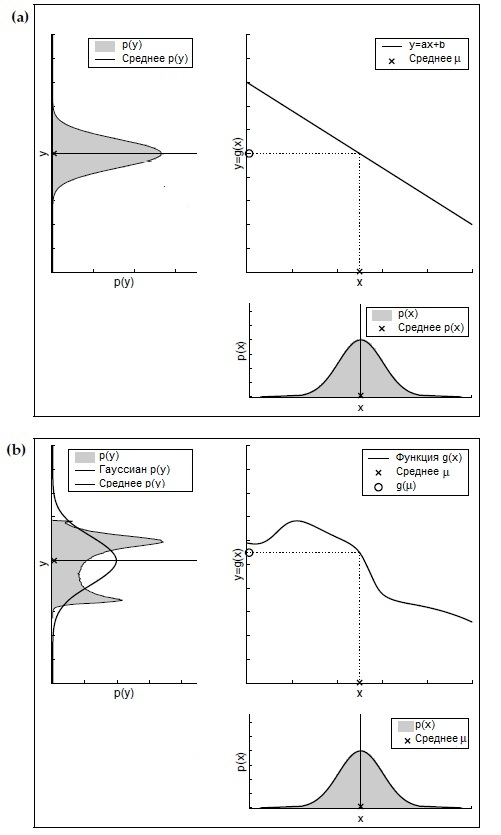
\includegraphics[width=0.9\linewidth]{33orig}}
	\caption{ (  Рис 3.3	Линейное (a) и нелинейное (b) преобразование случайной гауссовой переменной. На нижнем правом графике показана плотность начальной случайной переменной, $X$. Эта случайная переменная проходит через функцию, показанную на верхних правых графиках (пунктиром показано преобразование математического ожидания). Плотность результирующей случайной переменной $Y$ показана на верхних графиках слева.)}
	\label{fig:33orig}
\end{figure}
 
Эта модель строго обобщает линейное гауссово описание, лежащее в основе фильтров Калмана, как допускается выражениями (3.2) и (3.5). Функция $g$ заменяет матрицы $A_t$ и $B_t$ в (3.2), а $h$ - заменяет матрицу $C_t$ в (3.5). К сожалению, для произвольных функций $g$ и $h$ оценка больше не будет нормальным распределением. На практике, обновление оценки обычным образом с помощью нелинейных функций $g$ и $h$ часто невозможно, а решения в закрытом виде для байесовского фильтра нет.

На Рис. 3.3b показано воздействие нелинейного преобразования на случайную гауссову переменную. На графиках снизу справа и сверху справа показаны случайная переменная $X$ и нелинейная функция $g$, соответственно. Плотность преобразованной случайной переменной, $Y = g(X)$, обозначена серой зоной на верхнем левом графике Рис. 3.3b. Поскольку эта плотность не может быть вычислена в закрытом виде, оценочно извлечём 500000 элементов из $p(x)$, передадим функции $g$, а затем отразим на гистограмме в диапазоне значений $g$. Как видно, $Y$ нормальным распределением не является, в силу того, что нелинейности функции $g$ искажают плотность $X$.

Обобщенный фильтр Калмана (EKF) вычисляет гауссову аппроксимацию реальной оценки. Пунктиром на левом верхнем графике на Рис. 3.3b показано гауссово приближение плотности случайной переменной $Y$. Соответственно, EKF представляет оценку $bel(x_t)$ в момент времени $t$ в виде математического ожидания $\mu_t$ и ковариационной матрицы $\varSigma_t$. Таким образом, EKF наследуют от фильтра Калмана общее представление оценки, но отличается в том, что эта оценка лишь приближенная, а не точная, как в простых калмановских фильтрах. Таким образом, смысл EKF не в вычислении точной апостериорной вероятности, а в эффективной приближенной оценке ее математического ожидания и ковариации. Поскольку эти статистики не могут быть вычислены в закрытом виде, в алгоритме EKF необходимо прибегать к дополнительной аппроксимации.\\

\textbf{3.3.2 Линеаризация разложением в ряд Тейлора}\\

Ключевая идея в основе EKF называется \textit{линеаризацией}, общая концепция показана на Рис. 3.4. Линеаризация аппроксимирует нелинейную функцию $g$ с помощью касательной в точке математического ожидания гауссиана линейной функции (пунктирная линия на верхнем правом графике). Проекция гауссовой функции с помощью линейной аппроксимации даёт, в результате, плотность, что показано пунктирной линией на верхнем левом графике. Сплошной линией показаны математическое ожидание и ковариация после аппроксимации методом Монте-Карло. Разница между этими двумя гауссианами составляет ошибку, вызванную линейной аппроксимацией функции $g$.

Ключевым преимуществом линеаризации является ее эффективность.    

\begin{figure}[H]
	\center{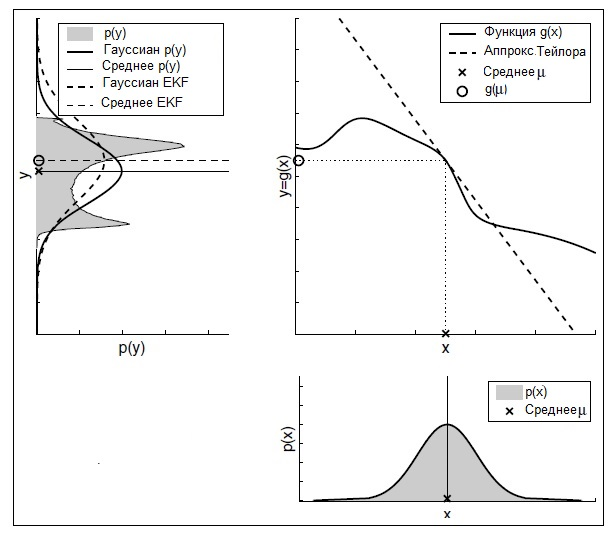
\includegraphics[width=0.9\linewidth]{34orig}}
	\caption{ (  Рис. 3.4 Иллюстрация линеаризации, применяемой для EKF. Вместо представления гауссовой функции через нелинейную функцию $g$ производится линейная аппроксимация $g$ с помощью касательной в точке математического ожидания линейной функции. Результирующая гауссова функция показана пунктиром на левом верхнем графике. Линеаризация влечёт за собой ошибку приближения, наблюдаемую в виде разницы между линеаризованной гауссовой функцией (пунктирной) и гауссианом, вычисленным с помощью точной оценки методом Монте-Карло (сплошная линия).)}
	\label{fig:34orig}
\end{figure} 
	
Оценка гауссовской функции методом Монте-Карло была получена заданием 500000 точек функции $g$ с последующим вычислением математического ожидания и ковариации. С другой стороны, линеаризация, применяемая в EKF, требует лишь определения линейного приближения с последующим вычислением результирующей гауссовой функции в закрытом виде. Фактически, после линеаризации $g$, механика распространения оценки в EKF и фильтрах Калмана одинакова.

Этот метод применим также при перемножении гауссовых функций, когда участвует функция измерения $h$. И снова в EKF выполняется приближение $h$ с помощью касательной линейной функции для сохранения нормального распределения апостериорной оценки.

РАЗЛОЖЕНИЕ В РЯД ТЕЙЛОРА

Существует множество методов для линеаризации нелинейных функций. В EKF используется способ, называемый \textit{разложением в ряд Тейлора} (первого порядка). Разложение в ряд Тейлора создаёт линейное приближение функции $g$ на основании её значения и наклона. Наклон задаётся частной производной\\

(3.50)
$$g'(u_t,x_{t-1}):=\frac{\partial g(u_t,x_{t-1})}{\partial x_{t-1}}$$

Разумеется, и значение $g$, и наклон зависят от аргументов функции. Логичным выбором аргумента является состояние, которое, вероятнее всего, наступит на момент линеаризации. Для гауссовых функций наиболее вероятное состояние - среднее апостериорной вероятности $\mu_{t-1}$ (математическое ожидание). Другими словами, функция $g$ аппроксимируется по значению в $\mu_{t-1}$ (и $u_t$), а линейная экстраполяция достигается с помощью коэффициента, пропорционального градиенту $g$ для $\mu_{t-1}$ и $u_t$:\\

(3.51)
$$g(u_t,x_{t-1})\approx g(u_t,\mu_{t-1})+\underbrace{g'(u_t,\mu_{t-1})}_{=:G_t}(x_{t-1}-\mu_{t-1})$$

$\hspace{32mm}=g(u_t,\mu_{t-1})+G_t(x_{t-1}-\mu_{t-1})$\\

Записанная в виде гауссовой функции, переходная вероятность в приближенном виде выглядит следующим образом:\\

(3.52)
$$p(x_t|u_t,x_{t-1})\approx\det(2\pi R_t)^{-\frac{1}{2}}\exp\{-\frac{1}{2}[x_t-g(u_t,\mu_{t-1})-G_t(x_{t-1}-\mu_{t-1})]^T$$

$\hspace{23mm}R_t^{-1}[x_t-g(u_t,\mu_{t-1})-G_t(x_{t-1}-\mu_{t-1})]\}$\\

ЯКОБИАН\\
Заметим, что $G_t$ – матрица размера $n\times n$, где $n$ означает размерность состояния. Такая матрица часто называется \textit{якобианом}. Значение якобиана зависит от $u_t$ и $\mu_{t-1}$, и, поэтому, различается для разных моментов времени.

В EKF используется аналогичная линеаризация для функции измерения $h$. Здесь разложение в ряд Тейлора происходит по $\bar{\mu}_t$, наиболее вероятному состоянию, определённому роботом в момент линеаризации по $h$:\\

(3.53)
$$h(x_t)\approx h(\bar{\mu}_t)+\underbrace{h'(\bar{\mu}_t)}_{=:H_t}(x_t-\bar{\mu}_t)$$
$\hspace{45mm}=h(\bar{\mu}_t)+H_t(x_t-\bar{\mu}_t)$\\

С частной производной $h'(x_t)=\frac{\partial h(x_t)}{\partial x_t}$ и в виде гауссовой функции, получим\\

(3.54)
$$p(z_t|x_t)=\det(2\pi Q_t)^{-\frac{1}{2}}\exp\{-\frac{1}{2}[z_t-h(\bar{\mu}_t)-H_t(x_t-\bar{\mu}_t)]^T$$
$\hspace{32mm}Q_t^{-1}[z_t-h(\bar{\mu}_t)-H_t(x_t-\bar{\mu}_t)]\}$\\


\begin{table}[H]
\begin{center}
\begin{tabular}{|l|}
\hline
1: \hspace{3mm} Algorithm Extended\_Kalman\_filter $(\mu_{t-1},\varSigma_{t-1},u_t,z_t):$ \\
{}\\
2: \hspace{7mm} 
$\bar{\mu}_t=g(u_t,\mu_{t-1})$\\
3: \hspace{7mm} $\bar{\varSigma}_t=G_t \varSigma_{t-1}G_t^T+R_t$\\
4: \hspace{7mm} $K_t=\bar{\varSigma}_t H_t^T(H_t\bar{\varSigma}_t H_t^T+Q_t)^{-1}$\\
5: \hspace{7mm} $\mu_t=\bar{\mu}_t+K_t(z_t-h(\bar{\mu}_t))$\\
6: \hspace{7mm}  $\varSigma_t=(I-K_t H_t)\bar{\varSigma}_t$\\
7: \hspace{7mm}
\textit{return} $\mu_t,\varSigma_t$\\
{}\\
\hline
\end{tabular}
\caption{(Таблица 3.3 Алгоритм обобщённого фильтра Калмана. )}
\end{center}
\end{table}

\textbf{3.3.3 Алгоритм EKF}\\
 
В Таблице 3.3 приводится \textit{алгоритм обобщённого фильтра Калмана}. Во многих отношениях, этот алгоритм похож на алгоритм калмановского фильтра, приведённый в Таблице 3.1. Наиболее важные различия указаны в следующей таблице:\\

\begin{table}[H]
\begin{center}
\begin{tabular}{l|c|c}
{}&Фильтр Калмана& EKF\\
\hline
прогноз состояния (строка 2)& $A_t\mu_{t-1}+B_t u_t$ & $g(u_t,\mu_{t-1})$ \\
прогноз измерения (строка 5)& $C_t\bar{\mu}_t$ & $h(\bar{\mu}_t)$
\end{tabular}
\end{center}
\end{table} 

Таким образом, линейные прогнозы калмановских фильтров заменяются в EKF нелинейными обобщениями. Более того, вместо системы линейных  матриц $A_t$, $B_t$, и $C_t$, используемой в калмановских фильтрах, в алгоритме EKF использованы якобианы $G_t$ и $H_t$, соответственно. Якобиан $G_t$ соответствует матрицам $A_t$ и $B_t$, а якобиан $H_t$ - матрице $C_t$. Обобщённые калмановские фильтры будут детально разобраны на примерах в Главе 7.\\

\textbf{3.3.4 Математический вывод для EKF}\\

Математический вывод EKF аналогичен выводу для фильтра Калмана в подразделе 3.2.4, поэтому, приводится в сокращённом виде. Прогноз вычисляется следующим образом (см. (3.8)):\\

(3.55)
$$\overline{bel}(x_t)=\int\underbrace{p(x_t|x_{t-1},u_t)}_{\sim N(x_t;g(u_t,\mu_{t-1})+G_t(x_{t-1}-\mu_{t-1}),R_t)}\underbrace{bel(x_{t-1})}_{\sim N(x_{t-1};\mu_{t-1},\varSigma_{t-1})} dx_{t-1}$$
 	
Это распределение для EKF является аналогом прогнозного распределения калмановского фильтра, приведённом в (3.8). Гауссова функция $p(x_t | x_{t-1},u_t)$ приводится в выражении (3.52). Функция $L_t$ задана с помощью (см. (3.11))\\

(3.56)
$$L_t=\frac{1}{2}(x_t-g(u_t,\mu_{t-1})-G_t(x_{t-1}-\mu_{t-1}))^T$$

$\hspace{29mm}R_t^{-1}(x_t-g(u_t,\mu_{t-1})-G_t(x_{t-1}-\mu_{t-1}))$\\

$\hspace{29mm}+\frac{1}{2}(x_{t-1}-\mu_{t-1})^T \varSigma_{t-1}^{-1}(x_{t-1}-\mu_{t-1})$

и является квадратичной как по $x_{t-1}$, так и по $x_t$, что указано выше. По аналогии с (3.12), разложим $L_t$ на $L_t(x_{t-1},x_t)$ и $L_t(x_t)$:\\

(3.57)
$$L_t(x_{t-1},x_t)=\frac{1}{2}(x_{t-1}-\varPhi_t[G_t^T R_t^{-1}(x_t-g(u_t,\mu_{t-1})+G_t\mu_{t-1})+\varSigma_{t-1}^{-1}\mu_{t-1}])^T \varPhi^{-1}$$

$\hspace{17mm}(x_{t-1}-\varPhi_t[G_t^T R_t^{-1}(x_t-g(u_t,\mu_{t-1})+G_t\mu_{t-1})+\varSigma_{t-1}^{-1}\mu_{t-1}])$

где\\

(3.58)
$$\varPhi_t=(G_t^T R_t^{-1}G_t+\varSigma_{t-1}^{-1})^{-1}$$

следовательно,\\

(3.59)
$$L_t(x_t)=\frac{1}{2}(x_t-g(u_t,\mu_{t-1})+G_t\mu_{t-1})^T R_t^{-1}(x_t-g(u_t,\mu_{t-1})+G_t \mu_{t-1})$$

$\hspace{15mm}+\frac{1}{2}(x_{t-1}-\mu_{t-1})^T \varSigma_{t-1}^{-1}(x_{t-1}-\mu_{t-1})$\\

$\hspace{15mm}-\frac{1}{2}[G_t^T R_t^{-1}(x_t-g(u_t,\mu_{t-1})+G_t\mu_{t-1})+\varSigma_{t-1}^{-1}\mu_{t-1}]^T$\\

$\hspace{15mm}\varPhi_t[G_t^T R_t^{-1}(x_t-g(u_t,\mu_{t-1})+G_t\mu_{t-1})+\varSigma_{t-1}^{-1}\mu_{t-1}]$\\

Как читатель может легко удостовериться, обнуление первой производной $L_t(x_t)$ даст функцию обновления вида $\mu_t = g(u_t,\mu_{t-1})$, по аналогии с выводом выражений с (3.27) по (3.31). Вторая производная задана $(R_t + G_t\varSigma_{t-1} G_t^T)^{-1}$ (см. (3.32)).

Обновление измерения выводится так же, как и для фильтра Калмана в Главе 3.2.4. По аналогии с (3.33), для EKF получается\\

(3.60)
$$bel(x_t)=\,\eta\underbrace{p(z_t|x_t)}_{\sim N(z_t;h(\bar{\mu}_t)+H_t(x_t-\bar{\mu}_t),Q_t)}\underbrace{\overline{bel}(x_t)}_{\sim N(x_t;\bar{\mu}_t,\bar{\varSigma}_t)}$$

Используем линеаризованую функцию перехода состояния из (3.53), что даёт следующую экспоненту (см. (3.35))\\

(3.61)
$$J_t=\frac{1}{2}(z_t-h(\bar{\mu}_t)-H_t(x_t-\bar{\mu}_t))^T Q_t^{-1}(z_t-h(\bar{\mu}_t)-H_t(x_t-\bar{\mu}_t))$$\\

$\hspace{15mm}+\frac{1}{2}(x_t-\bar{\mu}_t)^T \bar{\varSigma}_t^{-1}(x_t-\bar{\mu}_t)$\\

Получившиеся в результате математическое ожидание и ковариация заданы в виде\\

(3.62)
$$\mu_t=\bar{\mu}_t+K_t(z_t-h(\bar{\mu}_t))$$

(3.63)
$$\varSigma_t=(I-K_t H_t)\bar{\varSigma}_t$$

а калмановское усиление равно\\

(3.64)
$$K_t=\bar{\varSigma}_t H_t^T(H_t\bar{\varSigma}_{t-1}H_t^T+Q_t)^{-1}$$

Вывод этих равенств аналогичен последовательности выражений с (3.36) по (3.47).\\

\textbf{3.3.5 Практические соображения}\\

EKF стал едва ли не самым популярным инструментом оценки состояния в робототехнике. Его сильными сторонами является простота и вычислительная эффективность. Как и для фильтров Калмана, каждое обновление требует времени $O(k^{2.4} + n^2)$, где $k$ – размерность вектора измерений $z_t$, а $n$ – размерность вектора состояний $x_t$. Другие алгоритмы, например, обсуждаемые ниже многочастичные фильтры, могут потребовать времени, экспоненциально зависящего от $n$.

Вычислительная эффективность EKF основана на факте представления оценки с помощью многомерного гауссового распределения. Гауссова функция представляет собой одномодальное распределение, которое можно считать единственной догадкой с неопределённостью в виде эллипса. Нормальные распределения являются надёжными функциями оценки для многих практических задач и, скажем, использование калмановского фильтра на пространствах состояний от 1000 и более измерений ещё будет обсуждаться. EKF с большим успехом были использованы в ряде задач оценки состояния с нарушениями указанных допущений.

Важное ограничение EKF возникает в силу аппроксимации перехода состояний и измерений с использованием линейных разложений в ряд Тейлора. Для большинства задач робототехники переходы между состояниями и измерениями нелинейны, в результате, качество применяемой в EKF линейной аппроксимации зависит от двух основных факторов:  неопределённости и  локальной нелинейности аппроксимируемых функций. На двух графиках на Рис. 3.5 показана зависимость от неопределённости. На них две случайные гауссовы переменные пропускаются через одну и ту же нелинейную функцию (также см. Рис. 3.4). Хотя обе гауссовы функции имеют одинаковое математическое ожидание, переменная, показанная на графике (a) имеет более высокую степень неопределённости по сравнению с (b).\\
\begin{figure}[H]
	\center{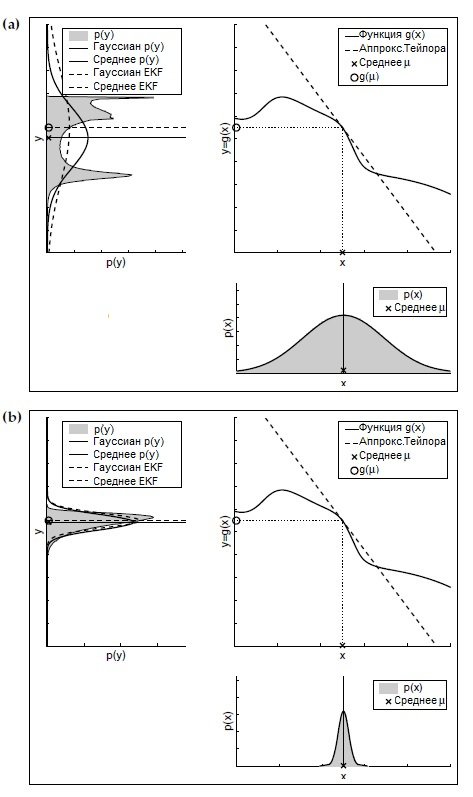
\includegraphics[width=0.8\linewidth]{35orig}}
	\caption{ (  Рис. 3.5 Зависимость качества аппроксимации от степени неопределённости. Обе гауссовы функции (справа снизу) имеют одинаковое математическое ожидание и подаются на одну и ту же нелинейную функцию (сверху справа). Большая неопределённость левой гауссовой функции даёт, в результате, более искажённое распределение плотности результирующей случайной переменной (серая область слева сверху). Сплошными линиями на графиках слева сверху показаны функции плотностей. Пунктиром обозначены гауссовы функции, полученные в результате линеаризации EKF.)}
	\label{fig:35orig}
\end{figure}  
Поскольку разложение в ряд Тейлора зависит только от математического ожидания, обе гауссовы функции проходят одинаковую линейную аппроксимацию. Закрашенные серым области на графике слева сверху обозначают плотности результирующей случайной переменной, вычисленной с помощью оценки методом Монте-Карло. Плотность, выраженная более широкой гауссовой кривой, значительно более искажена. Нормальные приближения плотностей показаны на схемах сплошными линиями, пунктиром обозначены линеаризации. Сравнение гауссовых функций, полученных в результате аппроксимации методом Монте-Карло, показывает, что большая степень неопределённости обычно ведёт к менее точной оценке математического ожидания и ковариации результирующей случайной переменной.

Второй фактор, влияющий на качество линейного приближения гауссовых функций, и показанный на Рис. 3.6, это локальная нелинейность функции $g$. Две гауссовы функции с одинаковой дисперсией проходят через одну нелинейную функцию. На схеме (a), математическое ожидание гауссовой функции попадает в диапазон функции $g$ с большей степенью нелинейности по сравнению с изображённой на графике (b). Разница между точной оценкой гауссовой функции методом Монте-Карло (сплошная линия, сверху слева) и полученной в результате линейной аппроксимации (пунктирная линия) показывает, что более высокая нелинейность влечёт возрастание ошибки аппроксимации. Совершенно очевидно, что в гауссовой функции EKF  размах получившейся плотности недооценивается.

Иногда необходимо иметь дело с несколькими отдельными гипотезами. Например, у робота может быть две отдельные гипотезы относительно своего местонахождения, но среднее арифметическое этих гипотез не выглядит правдоподобным. Для таких ситуаций требуется мультимодальные представления апостериорной оценки, неприменимые для EKF в описанном виде. Обычным обобщением EKF является отображение апостериорных вероятностей, в виде смеси (или суммы) гауссовых функций.\\
СМЕСЬ ГАУССОВЫХ ФУНКЦИЙ\\ 
Сумма гауссовых функций может иметь вид\\

(3.65)
$$bel(x_t)=\frac{1}{\varSigma_l \psi_{t,l}}\sum_l \psi_{t,l}\det(2\pi\varSigma_{t,l})^{-\frac{1}{2}}\exp\left\lbrace -\frac{1}{2}(x_t-\mu_{t,l})^T \varSigma_{t,l}^{-1}(x_t-\mu_{t,l})\right\rbrace$$

EKF С НЕСКОЛЬКИМИ ГИПОТЕЗАМИ\\
Здесь $\psi_{t,l}$ – это смесь параметров, где  $\psi_{t,l}\geq 0$. Эти параметры служат весами компонентов смеси. Они оцениваются на основе подобия наблюдений для соответствующих гауссовых функций. EKF, в которых используются такие представления в виде смесей называются \textit{обобщёнными фильтрами Калмана с несколькими гипотезами} или MHEKF.

Подводя итог, в случае, если нелинейные функции приблизительно линейны в области среднего значения оценки, то аппроксимация EKF будет, в общем, хорошим выбором для вычисления апостериорной оценки с удовлетворительной точностью. 
\begin{figure}[H]
	\center{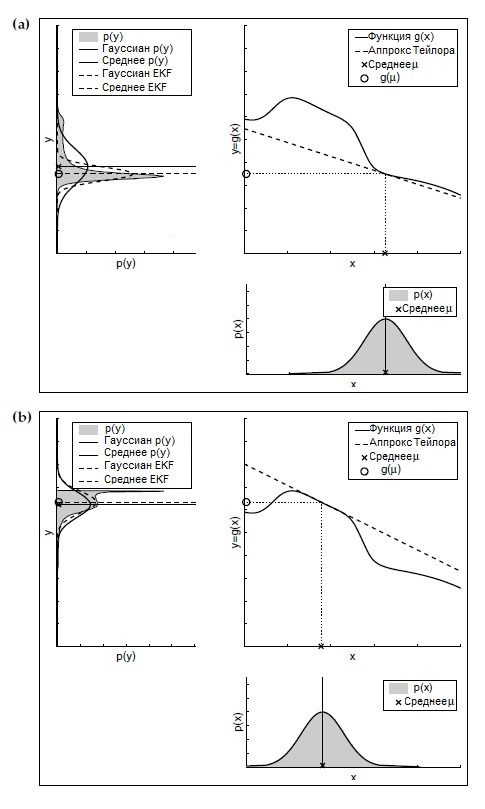
\includegraphics[width=0.8\linewidth]{36orig}}
	\caption{ (  Рис. 3.6 Зависимость качества аппроксимации от локальной нелинейности функции $g$. Обе гауссовы функции (изображены внизу справа на обоих схемах) имеют одинаковую ковариацию и передаются через одну и ту же функцию (вверху справа). Линейная аппроксимация, применяемая в EKF, показана пунктиром на графиках справа сверху. Сплошные линии на графиках слева сверху обозначают гауссовы функции, полученные из высокоточных оценок по методу Монте-Карло. Пунктирными линиями обозначены гауссовы функции, сгенерированные в результате линеаризации с помощью EKF.)}
	\label{fig:36orig}
\end{figure} 
Более того, чем меньше степень уверенности робота, тем шире будет гауссова оценка, и тем сильнее она подвержена нелинейности переходных функций  состояний и измерений. На практике, когда применяются EKF, важно следить за тем, чтобы неопределённость оценки состояния оставалась мала.\\

\textbf{3.4 Unscented Kalman Filter}\\

Разложение в ряд Тейлора, применяемое для EKF, является не единственным способом линеаризации преобразования гауссовой функции. Были найдены два других подхода, которые дают лучшие результаты. Один известен, как \textit{выравнивание моментов} (moments matching) (а фильтр известен под названием \textit{фильтр предполагаемой плотности} (assumed density filter - ADF)), в котором линеаризация вычислена так, чтобы сохранить настоящее значение математического ожидания и ковариации апостериорного распределения (чего не происходит в случае EKF). Другой метод линеаризации использован в unscented Kalman filter, или UKF, который выполняет стохастическую линеаризацию, используя процесс взвешенной статистической линейной регрессии. Обсудим UKF без математического вывода.\\
Unscented Kalman Filter\\ 
Мы призываем читателя более детально ознакомиться с темой, воспользовавшись библиографическим примечанием.\\

\textbf{3.4.1 Линеаризация с помощью Unscented преобразования}\\

На Рис. 3.7 показана линеаризация, которая используется в UKF, под названием \textit{unscented преобразование}. Вместо приближения функции $g$ с помощью разложения в ряд Тейлора\\
СИГМА ТОЧКА\\
UKF предопределенным образом извлекает так называемые сигма-точки гауссовой кривой и передаёт их функции $g$. В общем случае, эти сигма-точки расположены на среднем значении и симметричны вдоль главных осей ковариации (по две на измерение). Для $n$-мерного гауссиана с математическим ожиданием $\mu$ и ковариацией $\varSigma$, в результате получается $2n + 1$ сигма- точек $\mathcal X^{[i]}$, выбранных согласно следующему правилу:\\

(3.66)
$$\mathcal X^{[0]}=\mu$$

$\hspace{35mm}\mathcal X^{[i]}=\mu+\left( \sqrt{(n+\lambda)\varSigma}\right) _{i}$ \qquad\mbox {для $i=1,...,n$} 

$\hspace{35mm}\mathcal X^{[i]}=\mu-\left( \sqrt{(n+\lambda)\varSigma}\right) _{i-n}$ \qquad\mbox {для $i=n+1,...,2n$}
 
Здесь $\lambda=\alpha^2(n+\kappa)-n$, где $\alpha$ и $\kappa$ –параметры масштабирования, определяющие, как далеко сигма-точки отстоят от среднего значения. У каждой сигма-точки $\mathcal X^{[i]}$ имеется два связанных с нею веса. Один из весов, $\omega_m^{[i]}$, используется для вычисления математического ожидания, а другой, $\omega_c^{[i]}$, применяется при восстановлении ковариации гауссовой функции.\\

(3.67)
$$w_m^{[0]}=\frac{\lambda}{n+\lambda}$$

$\hspace{35mm}w_c^{[0]}=\frac{\lambda}{n+\lambda}+(1-\alpha^2+\beta)$\\

$\hspace{35mm}w_m^{[i]}=w_c^{[i]}=\frac{1}{2(n+\lambda)}$\qquad\mbox {для $i=1,...,2n$}\\

\begin{figure}[H]
	\center{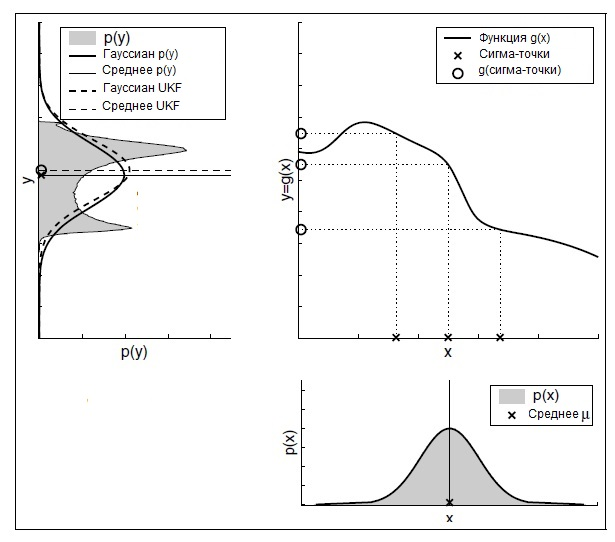
\includegraphics[width=1\linewidth]{37orig}}
	\caption{ (  Рис. 3.7 Иллюстрация линеаризации, применяемой в UKF. Сначала алгоритм фильтра  извлекает $2n + 1$ взвешенных сигма-точек из n-мерного гауссиана (в данном примере $n = 1$). Эти сигма-точки передаются нелинейной функции $g$. Из множества сигма-точек извлекается гауссова функция (показана маленькими кружками на правом верхнем графике). Аналогично EKF, линеаризация вызывает ошибку приближения, наблюдаемую в виде разницы между линеаризованной гауссовой функцией (пунктирная линия) и гауссианом, вычисленном с помощью высокоточной оценки методом Монте-Карло (сплошная линия). )}
	\label{fig:37orig}
\end{figure}

Параметр $\beta$ можно подобрать таким образом, чтобы закодировать дополнительные  данные более высокого порядка относительно распределения, лежащего в основе гауссовой функции. Для распределения, заданного точной гауссовой функцией, оптимальным выбором будет $\beta = 2$.

Затем сигма-точки передаются функции $g$, определяя, таким образом, изменение формы гауссиана.\\

(3.68)
$$\mathcal Y^{[i]}=g(\mathcal X^{[i]})$$

Параметры $(\mu'\,\varSigma')$ результирующей гауссовой функции извлекаются из помеченных сигма-точек $\mathcal Y^{[i]}$ в соответствии с\\

(3.69)
$$\mu'=\sum_{i=0}^{2n}w_m^{[i]}\mathcal Y^{[i]}$$

$\hspace{43mm}\varSigma'=\sum\limits_{i=0}^{2n}w_c^{[i]}(\mathcal Y^{[i]}-\mu')(\mathcal Y^{[i]}-\mu')^T$\\

На Рис. 3.8 показана зависимость unscented transform от степени неопределённости оригинальной гауссовой функции. Результаты разложения в ряд Тейлора для EKF для сравнения помещены на графике рядом с результатами преобразования UKF.

На Рис. 3.9 показано дополнительное сравнение между способами приближения UKF и EKF, в зависимости от локальной нелинейности функции $g$. Как легко заметить, unscented transform имеет большую точность по сравнению с разложением в ряд Тейлора первого порядка, используемое в EKF. Фактически, можно показать, что unscented transform дает точную оценку в пределах первых двух членов разложения Тейлора, а EKF охватывает только первый порядок. (Заметим, что и EKF, и UKF можно модифицировать для учёта членов более высоких порядков.)\\

\textbf{3.4.2 Алгоритм UKF}\\

Алгоритм UKF, использующий unscented transform представлен в Таблице 3.4. Формат входных и выходных данных аналогичен алгоритму EKF. В строке 2 с помощью равенства (3.66) определены сигма-точки предыдущей оценки, при этом $\gamma$ обозначает $\sqrt{n+\lambda}$. Эти точки передаются через алгоритм прогнозирования в строке 3, без учёта шумов. Затем прогнозируемые математическое ожидание и дисперсия вычисляются из результирующей совокупности сигма-точек (строки 4 и 5). Слагаемое $R_t$ в строке 5 добавляется к вычисленной с помощью сигма-точек ковариации с целью моделирования неопределённости, вносимой дополнительными  шумами прогнозирования (сравнимо со строкой 3 алгоритма EKF в Таблице 3.3). Шумы прогнозирования $R_t$ считаются аддитивными. Позже, в Главе 7, будет представлена версия алгоритма UKF, который выполняет более точную оценку прогнозируемых шумов и шумов измерений.

Новый набор сигма-точек извлекается из прогнозируемого гауссиана в строке 6. Этот набор  $\bar{\mathcal X}_t$ уже выражает общую неопределённость после такта прогнозирования. В строке 7 для каждой сигма-точки вычисляется прогнозируемое наблюдение. Результирующие сигма-точки наблюдения $\bar{\mathcal Z}_t$ используются для вычисления прогнозируемого наблюдения $\hat{z}_t$ и величины его неопределённости, $S_t$. Матрица $Q_t$ представляет собой ковариационную матрицу аддитивных шумов измерения. Заметим, что $S_t$ отображает ту же неопределённость, что и $H_t \bar{\varSigma}_t  H_t^T + Q_t$ в строке 4 алгоритма EKF. В строке 10 Таблицы 3.3 определяется взаимная ковариация между состоянием и наблюдением, которая затем используется в строке 11 для вычисления усиления фильтра Калмана $K_t$. Взаимная ковариация $\bar{\varSigma}_t^{x,z}$ соответствует члену $\bar{\varSigma}_t H)t^T$ в строке 4 алгоритма EKF. Учитывая все сказанное, легко показать, что обновление оценки, выполненное в строках 12 и 13, эквивалентно обновлению, выполняемому алгоритмом EKF.\\

\begin{figure}[H]
	\center{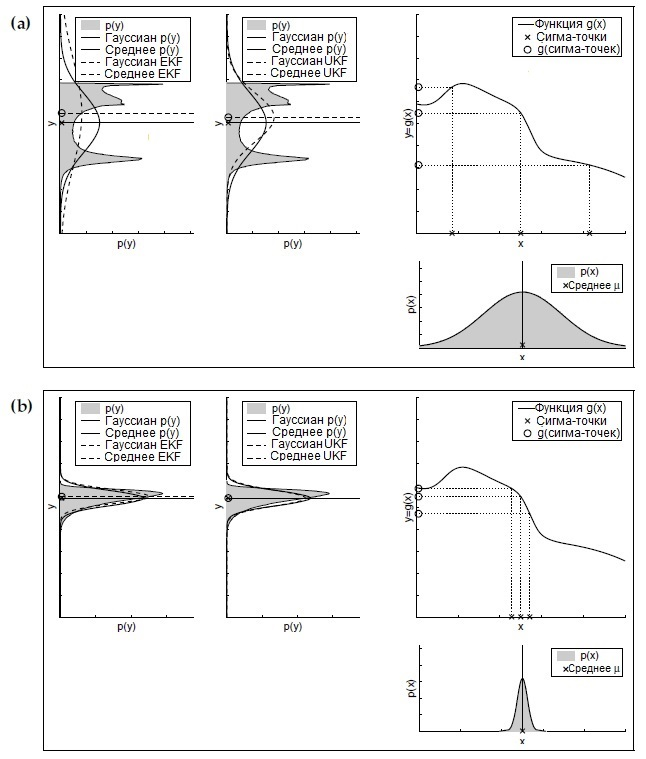
\includegraphics[width=1\linewidth]{38orig}}
	\caption{ (  Рис. 3.8 Результаты линеаризации для UKF в зависимости от неопределённости оригинальной гауссовой функции. Результаты линеаризации EKF показаны для сравнения на Рис. 3.5. Unscented transform имеет меньшую ошибку аппроксимации, что видно по заметной схожести между пунктирным и сплошным графиком гауссовых функций. )}
	\label{fig:38orig}
\end{figure}

\begin{figure}[H]
	\center{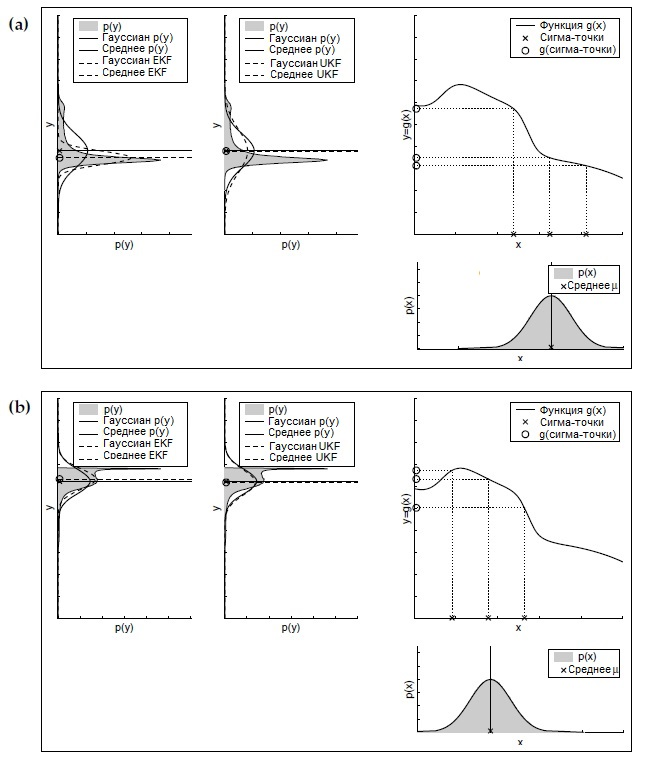
\includegraphics[width=1\linewidth]{39orig}}
	\caption{ (  Рис. 3.9 Результаты линеаризации UKF в зависимости от математического ожидания оригинальной гауссовой функции. Результаты линеаризации EKF также показаны для сравнения (см. Рис. 3.6). Линеаризация с помощью сигма-точек имеет меньшую ошибку аппроксимации, что видно по заметной схожести между пунктирным и сплошным графиком гауссовых функций. )}
	\label{fig:39orig}
\end{figure}

Асимптотическая сложность алгоритма UKF аналогична EKF. На практике EKF часто несколько быстрее, но алгоритм UKF остаётся очень эффективным, даже учитывая пропорциональное увеличение затрат времени. Более того, UKF наследует преимущества линеаризации unscented transform. Для чисто линейных систем будет показано, что оценки, сгенерированные с помощью UKF, идентичны оценкам калмановского фильтра.\\

\begin{table}[H]
\begin{center}
\begin{tabular}{|l|}
\hline
1: \hspace{3mm} Algorithm Unscented\_Kalman\_filter $(\mu_{t-1},\varSigma_{t-1},u_t,z_t):$ \\
{}\\
2: \hspace{7mm} 
$\mathcal X_{t-1}=(\mu_{t-1}\qquad\mu_{t-1}+\gamma\sqrt{\varSigma_{t-1}}\qquad\mu_{t-1}-\gamma\sqrt{\varSigma_{t-1}})$\\
3: \hspace{7mm} $\bar{\mathcal X}_t^{*}=g(u_t,\mathcal X_{t-1})$\\
4: \hspace{7mm} $\bar{\mu}_t=\sum\limits_{i=0}^{2n} w_m^{[i]}\bar{\mathcal X}_t^{*[i]}$\\
5: \hspace{7mm} $\bar{\varSigma}_t=\sum\limits_{i=0}^{2n}w_c^{[i]}(\bar{\mathcal X}_t^{*[i]}-\bar{\mu}_t)(\bar{\mathcal X}_t^{*[i]}-\bar{\mu}_t)^T+R_t$\\
6: \hspace{7mm}  $\bar{\mathcal X}_t=(\bar{\mu}_t\qquad\bar{\mu}_t+\gamma\sqrt{\bar{\varSigma}_t}\qquad\bar{\mu}_t-\gamma\sqrt{\bar{\varSigma}_t})$\\
7:  \hspace{8mm}$\bar{\mathcal Z}_t=h(\bar{\mathcal X}_t)$\\
8: \hspace{8mm}$\hat{z}_t=\sum\limits_{i=0}^{2n}w_m^{[i]}\bar{\mathcal Z}_t^{[i]}$\\
9: \hspace{8mm}$S_t=\sum\limits_{i=0}^{2n}w_c^{[i]}(\bar{\mathcal Z}_t^{[i]}-\hat{z}_t)(\bar{\mathcal Z}_t^{[i]}-\hat{z}_t)^T+Q_t$\\
10: \hspace{6mm}$\bar{\varSigma}_t^{x,z}=\sum\limits_{i=0}^{2n}w_c^{[i]}(\bar{\mathcal X}_t^{[i]}-\bar{\mu}_t)(\bar{\mathcal Z}_t^{[i]}-\hat{z}_t)^T$\\
11: \hspace{6mm}$K_t=\bar{\varSigma}_t^{x,z}S_t^{-1}$\\
12: \hspace{6mm}$\mu_t=\bar{\mu}_t+K_t(z_t-\hat{z}_t)$\\
13: \hspace{6mm}$\varSigma_t=\bar{\varSigma}_t-K_t S_t K_t^T$\\

14:\hspace{6mm}
\textit{return} $\mu_t,\varSigma_t$\\
{}\\
\hline
\end{tabular}
\caption{(Таблица 3.4 Алгоритм unscented Kalman filter. Переменная $n$ обозначает размерность вектора состояний.)}
\end{center}
\end{table}

Для нелинейных систем UKF даёт аналогичные или лучшие результаты по сравнению с EKF, при этом разница по отношению к EKF зависит от нелинейности и разброса неопределённости предыдущего состояния. Во многих практических реализациях разница между EKF и UKF ничтожна.

Другим преимуществом UKF является факт того, что они не требуют вычисления якобианов, которые, в некоторых случаях, трудно определить. В силу этого UKF часто называют \textit{фильтром без производных}.\\
ФИЛЬТР БЕЗ ПРОИЗВОДНЫХ

Наконец, unscented transform имеет некоторое сходство с представлением на основе выборки, используемом для многочастичного фильтра, которых будет обсуждаться в следующей главе. Однако, ключевое различие состоит в том, что сигма-точки в unscented transform точно определены, а в многочастичных фильтрах выборка выполняется случайным образом и приводит к важным последствиям. Если лежащее в основе распределение приближено к нормальному, тогда UKF представление значительно более эффективно по сравнению с представлением многочастичного фильтра. Если, с другой стороны, оценка очень далека от нормальной, тогда UKF представление слишком ограничено и фильтр плохо выполняет определение точек.\\

\textbf{3.5 Информационный фильтр}\\

Дополнением калмановского фильтра является \textit{информационный фильтр} (information filter- IF). Аналогично KF и его нелинейным версиям, EKF и UKF, информационный фильтр отображает оценку в виде гауссовой функции. Поэтому стандартный информационный фильтр использует те же допущения, что и фильтр Калмана. Ключевым различием между KF и IF является способ представления гауссовой оценки. Во всем семействе алгоритмов фильтров Калмана гауссовы функции представлены моментами (математическим ожиданием, ковариацией), а в информационных фильтрах – в каноническом представлении параметров, состоящем из информационной матрицы и информационного вектора. Разница параметризации приводит к разным уравнениям обновления. В частности, то, что вычислительно сложно в одном виде параметризации оказывается простым в другом (и наоборот). Каноническая параметризация и параметризация в виде моментов часто считаются взаимодополняющими, как и IF и KF.\\

\textbf{3.5.1 Каноническая параметризация}\\

КАНОНИЧЕСКАЯ ПАРАМЕТРИЗАЦИЯ\\
\textit{Каноническая параметризация} многомерной гауссовой функции задаётся матрицей $\varOmega$ и вектором $\xi$. Матрица $\varOmega$ – это инвертированная ковариационная матрица\\

(3.70)
$$\varOmega=\varSigma^{-1}$$

ИНФОРМАЦИОННАЯ МАТРИЦА\\
$\varOmega$ называется \textit{информационной матрицей}, или, иногда, \textit{матрицей точности}. Вектор $\xi$ называется \textit{информационным вектором}. Он определяется как\\

(3.71)
$$\xi=\varSigma^{-1}\mu$$

Легко заметить, что $\varOmega$ и $\xi$ образуют полную параметризацию гауссовой функции. В частности, математическое ожидание и ковариацию гауссовой функции можно легко получить из канонической параметризации путём инверсии (3.70) и (3.71):\\

(3.72)
$$\varSigma=\varOmega^{-1}$$

(3.73)
$$\mu=\varOmega^{-1}\xi$$

Каноническая параметризация часто выводится путём умножения экспоненты гауссовой функции. В (3.1), определим многомерное нормальное распределение следующим образом:\\

(3.74)
$$p(x)=\det(2\pi\varSigma)^{-\frac{1}{2}}\exp\left\lbrace -\frac{1}{2}(x-\mu)^T\varSigma^{-1}(x-\mu)\right\rbrace $$

Очевидная последовательность преобразований ведёт к следующей параметризации:\\

(3.75)
$$p(x)=\det(2\pi\varSigma)^{-\frac{1}{2}}\exp\left\lbrace -\frac{1}{2}x^T\varSigma^{-1}x+x^T\varSigma^{-1}\mu-\frac{1}{2}\mu^T\varSigma^{-1}\mu\right\rbrace$$

$\hspace{14mm}=\underbrace{\det(2\pi\varSigma)^{-\frac{1}{2}}\exp\left\lbrace-\frac{1}{2}\mu^T\varSigma^{-1}\mu\right\rbrace }_{\textit{const.}}\exp\left\lbrace -\frac{1}{2}x^T\varSigma^{-1}x+x^T\varSigma^{-1}\mu\right\rbrace$\\

Множитель, помеченный “const.” не зависит от целевой переменной $x$. Поэтому, его можно заменить нормализующим членом $\eta$.\\

(3.76)
$$p(x)=\eta\,\exp\left\lbrace -\frac{1}{2}x^T\varSigma^{-1}x+x^T\varSigma^{-1}\mu\right\rbrace $$

В таком виде удобнее использовать параметризацию в виде канонических параметров $\varOmega$ и $\xi$.\\

(3.77)
$$p(x)=\eta\,\exp\left\lbrace -\frac{1}{2}x^T\varOmega x+x^T\xi\right\rbrace $$

Во многих отношениях, каноническая параметризация более элегантна по сравнению с параметризацией в виде моментов. В частности, отрицательный логарифм гауссовой функции представляет собой квадратичную функцию в $x$, с каноническими параметрами $\varOmega$ и $\xi$:\\

(3.78)
$$-\log p(x)=\textit{const.}+\frac{1}{2}x^T\varOmega x-x^T\xi$$

Здесь "const." означает константу. Читатель может заметить, что мы не можем использовать символ $\eta$ для обозначения этой константы, поскольку отрицательные логарифмы вероятностей не нормализуются до 1. Отрицательный логарифм распределения $p(x)$ квадратичен по $x$, его квадратичный член параметризован по $\varOmega$, а линейный – по $\xi$. Фактически, для гауссовых функций $\varOmega$ должна быть неотрицательно полуопределена, поэтому $-\log p(x)$ является квадратичной функцией расстояния с математическим ожиданием $\mu=\varOmega^{-1}\xi$ £. Это легко проверяется установкой первой производной (3.78) в нуль:\\

(3.79)
$$\frac{\partial[-\log p(x)]}{\partial x}\,=\,0\,\Leftrightarrow\,\varOmega x-\xi\,=\,0\,\Leftrightarrow\,x=\varOmega^{-1}\xi$$\\

РАСCТОЯНИЕ МАХАЛАНОБИСА\\
Матрица $\varOmega$ определяет скорость, с которой возрастает функция расстояния в различных измерениях переменной $x$. Квадратичное расстояние, взвешенное матрицей $\varOmega$, называется \textit{расстоянием Махаланобиса}.\\

\begin{table}[H]
\begin{center}
\begin{tabular}{|l|}
\hline
1: \hspace{3mm} Algorithm Information\_filter $(\xi_{t-1},\varOmega_{t-1},u_t,z_t):$ \\
{}\\
2: \hspace{7mm} 
$\bar{\varOmega}_t=(A_t\varOmega_{t-1}^{-1}A_t^T+R_t)^{-1}$\\
3: \hspace{7mm} $\bar{\xi}_t=\bar{\varOmega}_t(A_t\varOmega_{t-1}^{-1}\xi_{t-1}+B_t u_t)$\\
{}\\
4: \hspace{7mm} $\varOmega_t=C_t^T Q_t^{-1}C_t+\bar{\varOmega}_t$\\
5: \hspace{7mm} $\xi_t=C_t^T Q_t^{-1}z_t+\bar{\xi}_t$\\
6: \hspace{7mm}
\textit{return} $\xi_t,\varOmega_t$\\
{}\\
\hline
\end{tabular}
\caption{(Таблица 3.5 Алгоритм информационного фильтра. )}
\end{center}
\end{table}

\textbf{3.5.2 Алгоритм информационного фильтра}\\


В Таблице 3.4 приводится модифицированный вариант алгоритма, который известен под названием \textit{«информационного фильтра»}. На вход подаётся нормальная гауссова функция в классическом представлении, заданная вектором  $\xi_{t-1}$ и матрицей   $\varOmega_{t-1}$ и определяющая оценку состояния в момент времени $t-1$. Аналогично всем байесовским фильтрам, входные данные включают векторы управляющего воздействия $u_t$ и измерения $z_t$. Выходными данными фильтра являются новые значения вектора $\xi_t$  матрицы $\varOmega_t$ и обновлённая гауссова функция, соответственно.

Этап обновления предусматривает использование матриц $ A_t $, $ B_t $, $ C_t $, $ R_t $, и $ Q_t $, описанных в Разделе 3.2. Алгоритм информационного фильтра основан на предположении о том, что вероятности перехода состояний и измерений могут быть выражены с помощью следующих гауссовых уравнений, впервые представленных в (3.2) и (3.5):\\

(3.80)
$$x_t=A_t x_{t-1}+B_t u_t+\varepsilon_t$$

(3.81)
$$z_t=C_t x_t+\delta_t$$

В данном случае, $ R_t $ и $ Q_t $, – это ковариации переменных нулевого среднего зашумления, $\varepsilon_t$ и $\delta_t$, соответственно.
 
Как и классический калмановский фильтр, информационный фильтр предусматривает обновление в две фазы, экстраполяции и коррекции. Фаза экстраполяции выполняется с помощью выражений в строках 2 и 3 Таблицы 3.4. Параметры $\bar{\xi}_t$ и $\bar{\varOmega}_t$ описывают гауссову функцию оценки по вектору состояний $ x_t $,  после учёта управляющего воздействия $ u_t $ , но до учёта измерений $ z_t $. Измерения принимаются во внимание в строках 4 и 5, где происходит обновление значений параметров оценки на основе измерений $ z_t $ в момент времени $ t $.

Эти две фазы обновления могут очень сильно различаться по сложности, особенно для случая, когда пространство состояний имеет большое число измерений. Как показано в Таблице 3.5, во время фазы экстраполяции происходит инверсия двух матриц размера $n\times n$, где $n$ – размерность пространства состояний. Инверсия матриц, по текущим оценкам, требует затрат времени, приблизительно $O(n^{2.4})$. Но для фильтров Калмана обновление имеет аддитивный характер и требует, максимум $O(n^2)$. Требуемое время ещё более уменьшается, если набор переменных зависит только от управляющего воздействия, или если перенос переменных выполняется независимо друг от друга. Для информационного фильтра ситуация обратная, поскольку в нем аддитивно происходит обновление измерений. Поэтому максимальные затраты времени также составят $ O(n^2) $, а эффективность  улучшится в случае, если измерения содержат только данные о наборе всех переменных состояния для конкретного момента времени. Обновление измерений в калмановских фильтрах очень затратно, из-за необходимости инверсии матриц, а вычислительная сложность, в худшем случае, достигает $O(n^{2.4})$. Это хорошо иллюстрирует взаимодополняющий характер калмановских и информационных фильтров.\\

\textbf{3.5.3 Математический вывод алгоритма информационного фильтра}\\

Вывод для информационного фильтра аналогичен выводу для фильтра Калмана.\\
ТАКТ ПРОГНОЗИРОВАНИЯ

Для математического вывода \textit{такта прогнозирования} (строки 2 и 3 в Таблице 3.5), начнём с соответствующих равенств обновления для калмановских фильтров которые находятся в строках 2 и 3 алгоритма в Таблице 3.1 и повторно приведены здесь для удобства читателя:\\

(3.82)
$$\bar{\mu}_t=A_t\mu_{t-1}+B_t u_t$$

(3.83)
$$\bar{\varSigma}_t=A_t\varSigma_{t-1}A_t^T+R_t$$

Далее в такте прогнозирования информационного фильтра производится замена моментов $\mu$ и $\varSigma$ каноническими параметрами $\xi$ и $\varOmega$, в соответствии с их определениями в (3.72) и (3.73):\\

(3.84)
$$\mu_{t-1}=\varOmega_{t-1}^{-1}\xi_{t-1}$$

(3.85)
$$\varSigma_{t-1}=\varOmega_{t-1}^{-1}$$

Подставка этих выражений в (3.82) и (3.83) даст набор равенств для прогнозирования\\

(3.86)
$$\bar{\varOmega}_t=(A_t\varOmega_{t-1}^{-1}A_t^T+R_t)^{-1}$$

(3.87)
$$\bar{\xi}_t=\bar{\varOmega}_t(A_t\varOmega_{t-1}^{-1}\xi_{t-1}+B_t u_t)$$
  
Эти равенства идентичны приведённым в Таблице 3.5. Легко заметить, что такт прогнозирования включает две вложенные инверсии потенциально больших матриц. Этих инверсий можно избежать, если обновление на такте движения  затрагивает только небольшое число переменных состояния, что будет обсуждаться чуть позже.\\ 
ОБНОВЛЕНИЕ ИЗМЕРЕНИЯ

Вывод для \textit{обновления измерения} ещё проще. Начнём с гауссовой функции оценки в момент времени t, упомянутой в уравнении (3.35) и повторённой здесь:\\

(3.88)
$$bel(x_t)=\eta\exp\left\lbrace -\frac{1}{2}(z_t-C_t x_t)^T Q_t^{-1}(z_t-C_t x_t)-\frac{1}{2}(x_t-\bar{\mu}_t)^T\bar{\varSigma}_t^{-1}(x_t-\bar{\mu}_t)\right\rbrace $$
 
Для гауссовых функций, представленных в канонической форме, распределение задано следующим образом: \\

(3.89)
$$bel(x_t)=\eta\exp\left\lbrace -\frac{1}{2}x_t^T C_t^T Q_t^{-1}C_t x_t+x_t^T C_t^T Q_t^{-1}z_t-\frac{1}{2}x_t^T\bar{\varOmega}_t x_t+x_t^T\bar{\xi}_t\right\rbrace $$

будучи переписанным в виде экспоненты, выражение разрешается как \\

(3.90)
$$bel(x_t)=\eta\exp\left\lbrace -\frac{1}{2}x_t^T[C_t^T Q_t^{-1}C_t+\bar{\varOmega}_t]x_t+x_t^T[C_t^T Q_t^{-1}z_t+\bar{\xi}_t]\right\rbrace $$

Сейчас можно окончательно сформулировать равенства обновления измерений, собрав все члены в квадратные скобки:\\

(3.91)
$$\xi_t=C_t^T Q_t^{-1}z_t+\bar{\xi}_t$$

(3.92)
$$\varOmega_t=C_t^T Q_t^{-1}C_t+\bar{\varOmega}_t$$

Эти равенства идентичны приведённым в строках 4 и 5, такта обновления измерения Таблицы 3.5.\\

\textbf{3.5.4 Алгоритм обобщённого информационного фильтра}\\

Обобщенный информационный фильтра (extended information – EIF), расширяет информационный фильтр для нелинейного случая, практически таким же образом, как EKF представляет собой нелинейное расширение фильтра Калмана. Алгоритм EIF приведён в Таблице 3.6. Прогнозирование выполняется в строках с 2 по 4, а обновление измерения - с 5 по 7. Эти уравнения такта обновления, по большей части, аналогичны линейному информационному фильтру, где функции $g$ и $h$ (и их якобианы $G_t$ и $H_t$) заменяют параметры линейной модели $A_t$, $B_t$, и $C_t$. Как и прежде, $g$ и $h$ обозначают нелинейные переходные функции состояния и измерения, соответственно. Они были впервые определены в (3.48) и (3.49) и повторно приводятся ниже:\\

(3.93)
$$x_t=g(u_t,x_{t-1})+\varepsilon_t$$

(3.94)
$$z_t=h(x_t)+\delta_t$$

К сожалению функции $g$ и $h$ принимают на вход данные о состоянии, что требует восстановления оценки состояния $\mu$ на основании канонических параметров. Восстановление выполняется в строке 2, в которой состояние $\mu_{t-1}$ очевидным образом вычисляется из $\varOmega_{t-1}$ и $\xi_{t-1}$. В строке 5 вычисляется состояние $\bar{\mu}_t$, используя уже знакомое по EKF выражение (строка 2 в Таблице 3.3). Кажется, что необходимость восстанавливать оценку состояния противоречит идее представления фильтра с каноническими параметрами. Мы вернёмся к этой теме при обсуждении использования обобщённых информационных фильтров в контексте построения карт для роботов.\\
 
\begin{table}[H]
\begin{center}
\begin{tabular}{|l|}
\hline
1: \hspace{3mm} Algorithm Extended\_ information\_filter $(\xi_{t-1},\varOmega_{t-1},u_t,z_t):$ \\
{}\\
2: \hspace{7mm} 
$\mu_{t-1}=\varOmega_{t-1}^{-1}\xi_{t-1}$\\
3: \hspace{7mm} $\bar{\varOmega}_t=(G_t\varOmega_{t-1}^{-1}G_t^T+R_t)^{-1}$\\
4: \hspace{7mm} $\bar{\xi}_t=\bar{\varOmega}_t g(u_t,\mu_{t-1})$\\
5: \hspace{7mm} $\bar{\mu}_t=g(u_t,\mu_{t-1})$\\
6: \hspace{7mm} $\varOmega_t=\bar{\varOmega}_t+H_t^T Q_t^{-1}H_t$\\
7: \hspace{7mm} $\xi_t=\bar{\xi}_t+H_t^T Q_t^{-1}[z_t-h(\bar{\mu}_t)+H_t\bar{\mu}_t]$\\
8: \hspace{7mm}
\textit{return} $\xi_t,\varOmega_t$\\
{}\\
\hline
\end{tabular}
\caption{(Таблица 3.6 Алгоритм расширенного информационного фильтра (EIF). )}
\end{center}
\end{table}

\textbf{3.5.5 Математический вывод обобщённого информационного фильтра}\\

Обобщённый информационный фильтр легко вывести, используя, в основном, ту же самую линеаризацию, которая была ранее использована для обобщённых фильтров Калмана. Как в (3.51) и (3.53), в обобщённом информационном фильтре с помощью разложения в ряд Тейлора оцениваются функции $g$ и $h$:\\

(3.95)
$$g(u_t,x_{t-1})\,\approx\,g(u_t,\mu_{t-1})+G_t(x_{t-1}-\mu_{t-1})$$

(3.96)
$$h(x_t)\,\approx\,h(\bar{\mu}_t)+H_t(x_t-\bar{\mu}_t)$$

здесь $G_t$ и $H_t$ - якобианы $g$ и $h$ для $\mu_{t-1}$ и $\bar{\mu}_t$, соответственно:\\

(3.97)
$$G_t=g'(u_t,\mu_{t-1})$$

(3.98)
$$H_t=h'(\bar{\mu}_t)$$
 
Эти определения аналогичны используемым в EKF. Выражения для такта экстраполяции выводятся из строк 2 и 3 алгоритма EKF (Таблица 3.3), которые приведены ниже:\\

(3.99)
$$\bar{\varSigma}_t=G_t\varSigma_{t-1}G_t^T+R_t$$

(3.100)
$$\bar{\mu}_t=g(u_t,\mu_{t-1})$$

Замена $\varSigma_{t-1}$ на $\varOmega_{t-1}^{-1}$ и $\bar{\mu}_t$ на $\bar{\varOmega}_t^{-1}\xi_t$
даёт уравнения экстраполяции для расширенного информационного фильтра:\\

(3.101)
$$\bar{\varOmega}_t=(G_t\varOmega_{t-1}^{-1}G_t^T+R_t)^{-1}$$

(3.102)
$$\bar{\xi}_t=\bar{\varOmega}_t g(u_t,\varOmega_{t-1}^{-1}\xi_{t-1})$$
 
Обновление измерения выводится из уравнений (3.60) и (3.61). В частности, (3.61) определяет следующую апостериорную гауссову функцию:\\

(3.103)
$$bel(x_t)=\eta\exp\{ -\frac{1}{2}(z_t-h(\bar{\mu}_t)-H_t(x_t-\bar{\mu}_t))^T Q_t^{-1}$$

$\hspace{30mm}(z_t-h(\bar{\mu}_t)-H_t(x_t-\bar{\mu}_t))-\frac{1}{2}(x_t-\bar{\mu}_t)^T\bar{\varSigma}_t^{-1}(x_t-\bar{\mu}_t)\} $

Умножение экспоненты и переопределение членов даёт следующее выражение для апостериорной вероятности:\\

(3.104)
$$bel(x_t)=\eta\exp\{-\frac{1}{2}x_t^T H_t^T Q_t^{-1}H_t x_t+x_t^T H_t^T Q_t^{-1}[z_t-h(\bar{\mu}_t)+H_t\bar{\mu}_t]$$

$\hspace{18mm}-\frac{1}{2}x_t^T\bar{\varSigma}_t^{-1}x_t+x_t^T\bar{\varSigma}_t^{-1}\bar{\mu}_t\}$\\

$\hspace{15mm}=\eta\exp\{-\frac{1}{2}x_t^T[H_t^T Q_t^{-1}H_t+\bar{\varSigma}_t^{-1}]x_t$\\

$\hspace{18mm}+x_t^T[H_t^T Q_t^{-1}[z_t-h(\bar{\mu}_t)+H_t\bar{\mu}_t]+\bar{\varSigma}_t^{-1}\bar{\mu}_t]$

Учитывая, что $\bar{\varSigma}_t^{-1}=\bar{\varOmega}_t$, это выражение разрешается до следующего информационного вида:\\

(3.105)
$$bel(x_t)=\eta\exp\{-\frac{1}{2}x_t^T[H_t^T Q_t^{-1}H_t+\bar{\varOmega}_t]x_t$$

$\hspace{38mm}+x_t^T[H_t^T Q_t^{-1}[z_t-h(\bar{\mu}_t)+H_t\bar{\mu}_t]+\bar{\xi}_t]$

Сейчас можно сформулировать уравнения обновления измерения, собрав все члены в квадратных скобках:\\

(3.106)
$$\varOmega_t=\bar{\varOmega}_t+H_t^T Q_t^{-1}H_t$$

(3.107)
$$\xi_t=\bar{\xi}_t+H_t^T Q_t^{-1}[z_t-h(\bar{\mu}_t)+H_t\bar{\mu}_t]$$\\

\textbf{3.5.6 Практические соображения}\\

В контексте задач робототехники информационный фильтр имеет несколько преимуществ по сравнению с фильтром Калмана. Например, глобальное представление неопределённости в информационном фильтре достаточно простое: необходимо установить $\varOmega=0$. При использовании моментов, такие величины общей неопределённости дают ковариацию бесконечной степени. Это особенно проблематично, когда измерения датчиков несут информацию об ограниченном наборе всех переменных состояния, что часто встречается в робототехнике. Для решения таких ситуаций средствами EKF необходимо предпринимать дополнительные действия. Многие реализации информационного фильтра, которые будут обсуждаться позже, демонстрируют более стабильные количественные характеристики по сравнению с калмановским фильтром.

Как мы увидим в следующих главах книги, информационный фильтр с несколькими дополнениями позволяют роботу интегрировать информацию без немедленного отражения её в вероятностном виде. Это может стать решающим преимуществом в сложных задачах оценки, включающих сотни или даже миллионы переменных. Для таких больших задач попытки интеграции по типу фильтра Калмана ведёт к серьёзным вычислительным трудностям, поскольку каждую новую порцию информации требуется распространить  в большой системе переменных.  С помощью соответствующих модификаций информационного фильтра возможно обойти эту проблему, локально добавив эту информацию в систему. Однако, это свойство \textit{нехарактерно} для простого информационного фильтра, обсуждаемого сейчас. В Главе 12 мы обсудим обобщения этого фильтра.

Другое преимущество информационного фильтра перед фильтром Калмана возникает в силу его естественной приспособленности для решения задачи нескольких роботов.  Такие задачи часто включают интеграцию показаний датчиков, которые собираются децентрализовано, что обычно выполняется с помощью теоремы Байеса. Будучи представлена в логарифмическом виде, теорема Байеса становится суммой. Как было сказано выше, канонические параметры информационных фильтров выражают вероятность в логарифмической форме, поэтому интеграция информации представляет собой суммированием данных с нескольких роботов. Сложение коммутативно, поэтому с помощью информационных фильтров часто возможно интегрировать информацию в произвольном порядке, с произвольными задержками и в полностью децентрализованной манере. Хотя то же самое возможно сделать, используя параметризацию в виде моментов (в конце концов, они выражают одну и ту же информацию), необходимо будет предпринять большие дополнительные усилия. Несмотря на это достоинство, применение информационных фильтров в системах из нескольких роботов остаётся, по большей части, не исследованным. Мы вернёмся к задаче нескольких роботов в Главе 12.

Обратной стороной преимуществ информационного фильтра является наличие важных ограничений. Основным недостатком обобщённого информационного фильтра можно считать необходимость восстанавливать оценку состояния для нелинейных систем на такте обновления. В представленном виде это потребует инверсии информационной матрицы. Вдобавок, информационные фильтры требуют дополнительных операций инверсии матриц на этапе экстраполяции. Для многих задач робототехники использование EKF не требует инверсии матриц сравнимого размера. Считается, что для пространств состояний с большим числом измерений информационный фильтр проигрывает фильтру Калмана по вычислительной сложности, что является одной из причин подавляющей популярности последнего. 

Как будет позже показано в книге, эти ограничения не обязательно применимы для задач, в которых информационная матрица имеет явную структуру. Во многих задачах робототехники взаимодействие переменных состояния локально, следовательно, информационная матрица разрежена. Эта разреженность \textit{не} соотносится с разреженностью матрицы ковариации.

Можно считать информационные фильтры  графами, в которых состояния соединены, когда соответствующие элементы вне главной диагонали информационной матрицы не равны нулю. Разреженные информационные матрицы соответствуют разреженным графам,\\
МАРКОВСКИЕ СЛУЧАЙНЫЕ ПОЛЯ \\
которые широко известны под названием \textit{марковских случайных полей}. Для таких полей имеется множество алгоритмов, эффективно выполняющих операции общей оценки и обновления с названиями наподобие \textit{«алгоритма распространения доверия» (loopy belief propagation)}. В ходе изложения мы столкнёмся с проблемой картографирования, в которой информационная матрица будет (относительно) разрежена, и разработаем обобщенный информационный фильтр, который будет существенно эффективнее как  фильтров Калмана, так и информационных фильтров с неразреженными матрицами.\\

\textbf{3.6 Вывод}\\

В этом разделе мы представили эффективные алгоритмы байесовских фильтров, которые выражают апостериорные оценки в виде многомерных гауссовых функций.  Было отмечено, что \\

• Гауссовы функции могут быть представлены двумя различными способами: параметризацией в виде моментов и канонической параметризацией. Параметризация в виде моментов состоит из математического ожидания (первый момент) и ковариации (второй момент) функции нормального распределения. Каноническая или обычная параметризация состоит из информационной матрицы и информационного вектора. Оба вида параметризации взаимно дополняют друг друга, и каждую можно восстановить из другой, с помощью инверсию матриц.\\

• Для обоих видов параметризации можно реализовать байесовские фильтры. При использовании параметризации в виде моментов получившийся фильтр называется фильтром Калмана. Дополнением фильтра Калмана является информационный фильтр, представляющий апостериорную вероятность с использованием канонической параметризации. Обновление фильтра Калмана на основе управляющего воздействия вычислительно просто, в то время, как учёт измерения более труден. Для информационного фильтра ситуация обратная, учёт измерения достаточно прост, но обновить фильтр на основе управляющего сигнала вычислительно сложно.\\

• Для вычисления правильной апостериорной вероятности в обоих фильтрах требуется соблюсти три условия. Во-первых, начальная оценка должна быть нормальным распределением. Во-вторых, переходная вероятность состояния должна выражаться функцией с линейным аргументом и добавлением независимого нормально распределенного зашумления. В третьих, то же справедливо для вероятности измерения: она должна иметь линейный аргумент с добавлением гауссового шума. Системы, отвечающие этим требованиям, называются линейными гауссовыми системами. \\

• Оба фильтра можно обобщить для нелинейных задач. Один из методов, описанных в этой главе, состоит в вычислении касательной к нелинейной функции. Касательные линейны, что позволяет использовать это в обоих фильтрах. Способ нахождения касательной называется разложением в ряд Тейлора и включает вычисление первой производной целевой функции с последующей оценкой её в определённой точке. Результатом этой операции является матрица, известная как якобиан, а получившиеся в результате фильтры называют «обобщенными».  

• Так называемый unscented Kalman filter использует другой метод линеаризации, который называется «unscented transform». Он вычисляет значения функции в нескольких выбранных точках, и выполняет линеаризованную аппроксимацию на основе полученных результатов. Этот фильтр может быть использован без необходимости вычисления якобианов, и, потому, часто именуется «фильтром без производных». Unscented Kalman filter эквивалентен фильтру Калмана для линейных систем, но часто более эффективен для нелинейных систем. Вычислительная сложность этого фильтра и обобщённого фильтра Калмана одинаковы.\\

• Точность разложения в ряд Тейлора и unscented transform зависит от двух факторов: степени нелинейности системы и ширины апостериорного распределения. Обобщённые фильтры обычно показывают хорошие результаты, когда состояние системы известно с относительно высокой точностью, и оставшаяся ковариация мала. Чем больше степень неопределённости, чем больше ошибка, вносимая линеаризацией.\\

• Одним из главных преимуществ гауссовых фильтров является их вычислительная эффективность: обновление требует времени, кратного размерности пространства состояний, что значительно лучше некоторых методов, описанных в следующей главе. Основным недостатком является ограничение применимости одномодальными гауссовыми распределениями.\\

• Обобщение гауссовых функций для мультимодальных апостериорных распределений известно под названием фильтра Калмана с несколькими гипотезами. Этот фильтр отображает апостериорную вероятность в виде смеси гауссовых функций, представляющих собой взвешенную сумму нормальных распределений. Специфика обновления этого фильтра требует механизмов разделения, слияния или отсечения отдельных гауссианов. Фильтры Калмана с несколькими гипотезами хорошо подходят, в частности, для задач с дискретной интеграцией данных, часто встречающихся в робототехнике.\\

• В случае многомерных гауссовых функций и фильтр Калмана, и информационный фильтр имеют взаимно обратные сильные и слабые стороны. Однако, калмановский фильтр и его нелинейное обобщение, обобщенный калмановский фильтр, значительно более популярны по сравнению с информационным фильтром.\\

Выбор материалов для этой главы основывается на самых популярных, на сегодняшний день, методах робототехники. Существует огромное количество вариантов и обобщений гауссовых фильтров,  предназначенных для обхода различных ограничений и недостатков конкретных реализаций.
 
Значительное число алгоритмов в этой книге основано на гауссовых фильтрах. Множество практических проблем робототехники требует использования обобщений, c разреженными структурами или факторизацией апостериорного распределения.\\

\textbf{3.7 Библиографические примечания}\\

Фильтры Калмана были отрыты Свирлингом (1958) и Калманом (1960). Обычно, они представляются как оптимальная функция оценки методом наименьших квадратов, и, реже, в качестве метода вычисления апостериорных распределений, хотя, при соответствующих допущениях, обе точки зрения идентичны. Есть множество великолепных учебников по калмановским и информационным фильтрам, включая работу Мэйбека (Maybeck, 1990) и Язвински (Jazwinsky -1970). На сегодняшний день развитие калмановских фильтров с включением данных было описано в работах Бар-Шалома и Фортманна (Bar-Shalom и Fortmann,1988), Бар-Шалома и Ли (Bar- Shalom и Li, 1998).\\

Лемму об обращении матриц можно найти в работе Голаба и Лоана (Golub и Loan,1986). Согласно Копперсмиту и Винограду (Coppersmith, Winograd,1990), инверсия матриц может быть выполнена за время $O(n^2,376)$. Этот результат стал самым заметным в серии работ по улучшению вычислительной сложности для алгоритма отбора переменных ниже $O(n^3)$ . Серия началась с основополагающей работы Страссена (Strassen, 1969), в которой он сформулировал алгоритм, требующий $O(n^2,807)$. Кавер и Томас (Cover и Thomas, 1991) выполнили обзор теории информации с акцентом на дискретные системы. Unscented Kalman filter был создан Юлиером и Ульманном (Julier и Uhlmann, 1997). Сравнение UKF и EKF в контексте различных задач оценки состояния можно найти в работе ван де Мерве (van der Merwe, 2004). Минка (Minka, 2001) выполнил работу по подбору моментов (moments matching) и допустимой фильтрации плотностей для гауссовых смесей.\\

\textbf{3.8 Упражнения}\\

1. В этом и последующих упражнениях требуется разработать фильтр Калмана для простой динамической системы: автомобиль с линейной динамикой двигается в линейной окружающей среде. Для простоты допустим, что $\varDelta t=1$. Положение автомобиля в момент $t$ задано функцией $x_t$A. Его скорость $\dot{x}_t$, ускорение - $\ddot{x}_t$. Допустим, ускорение  в каждый момент времени определяется случайно, согласно гауссовой функции с нулевым математическим ожиданием и ковариацией $\sigma^2=1$.\\

(a) Каков минимальный вектор состояний фильтра Калмана, чтобы результирующая система была марковской?\\

(b) Для полученного вектора состояний найти переходную вероятность состояния $p(x_t | u_t,x_{t-1})$. Подсказка: эта функция перехода будет состоять из линейных матриц $A$ и $B$, а ковариации зашумления $R$ (см. выражение (3.4) и Таблицу 3.1).\\

(c) Реализовать такт экстраполяции состояния для фильтра Калмана. Допустим, известно, что в момент времени $t = 0$, $x_0 = \dot{x}_0 = \ddot{x}_0 =0$. Вычислить распределения состояний для моментов времени $t = 1, 2,..., 5$.\\

ЭЛЛИПС НЕОПРЕДЕЛЁННОСТИ

(d) Для каждого значения $t$, изобразить точками на графике апостериорное распределение по $x$ и $\dot{x}$, где $x$ – горизонтальная, а $\dot{x}$ – вертикальная ось. Для каждого апостериорного распределения необходимо изобразить \textit{эллипс неопределённости}, представляющий собой эллипс из точек на расстоянии одного стандартного отклонения от среднего. Подсказка: Если нет доступа к математической библиотеке, можно найти эллипсы путём анализа характеристического значения матрицы ковариации.\\

(e) Что произойдёт с корреляцией между $x_t$ и $\dot{x}_t$ при $t\uparrow\infty$?\\

2. Добавим к фильтру Калмана измерения. Допустим, в момент времени $t$ возможно получить зашумленное наблюдение $x$. Предполагается, что датчик измеряет истинное местоположение, искажённое гауссовским шумом с ковариацией $\sigma^2=10$.\\

(a) Определить модель измерения. Подсказка: Необходимо определить матрицу $C$ и ещё одну матрицу $Q$ (см. выражение (3.6) и Таблицу 3.1).\\

(b) Реализовать обновление измерения. Допустим, в момент времени $t = 5$, наблюдается значение измерения $z = 5$. Указать параметры гауссовой функции до и после обновления KF. Изобразить на графике эллипс неопределённости до и после учёта измерения (выше показано, каким образом изобразить эллипс неопределённости).\\
3. В подразделе 3.2.4 был выведен такт экстраполяции для KF. Этот такт часто выводится с помощью Z –преобразования или преобразования Фурье, используя теорему свёртки. Заново вывести выражения для такта прогнозирования, используя преобразования. \textit{Примечание: Это упражнение требует знания преобразования свёртки, что выходит за пределы материала этой книги}.\\

4. В тексте было отмечено, что линеаризация EKF является приближением. Для того, чтобы выяснить качество аппроксимации, выполните следующее упражнение. Допустим, имеется мобильный робот, действующий в плоской среде. Его состояние описано координатами его местоположения $x-y$ и глобальным направлением ориентации $\theta$. Допустим, с высокой степенью определённости известны $x$ и $y$, но неизвестна ориентация $\theta$. Это отражается следующей первоначальной оценкой \\

\begin{minipage}{0.3\textwidth}
	\begin{equation*}
	\mu=
	\left(\begin{array}{ccc}
	0 & 0 & 0\\
	\end{array}\right)
	\end{equation*}
\end{minipage}
\begin{minipage}{0.3\textwidth}
	\begin{equation*}
	\mbox {и} \hspace{10mm} \varSigma=
	\left(\begin{array}{ccc}
	0,01 & 0 & 0\\
	0 & 0,01 & 0\\
	0 & 0 & 10000\\
	\end{array}\right)
	\end{equation*}
\end{minipage}\\


Графически изобразить лучшую модель апостериорного распределения для положения робота в момент после передвижения робота на $d =1$ единиц вперёд. Для этого упражнения предположим, что робот движется плавно и без зашумления. Отсюда, прогнозируемое положение робота после движения будет\\

\begin{minipage}{0.3\textwidth}
	\begin{equation*}
	\left(\begin{array}{c}
	x'\\
	y'\\
	\theta'\\
	\end{array}\right)
	\end{equation*}
\end{minipage}
\begin{minipage}{0.3\textwidth}
	\begin{equation*}
	\mbox {=} \hspace{10mm} 
	\left(\begin{array}{c}
	x+\cos\theta\\
	y+\sin\theta\\
	\theta\\
	\end{array}\right)
	\end{equation*}
\end{minipage}\\


На графике можно опустить $\theta$, изобразив только апостериорное распределение для координат $x-y$.\\

(b) Учесть это движение в такте обновления EKF. Для этого необходимо определить функцию перехода состояний и линеаризовать ее. Затем необходимо сгенерировать новую гауссову оценку положения робота, используя линеаризованную модель. Необходимо дать точные математические равенства для каждого такта и определить результирующий гауссиан.\\
 
(c) Изобразить эллипс неопределённости гауссовой функции и сравнить его с интуитивным решением.\\
 
(d) Добавить в модель измерение. Пусть измерением будет зашумлённая проекция координаты $x$ робота с ковариацией $Q = 0,01$. Необходимо определить модель измерения. Затем применить измерение к найденному апостериорному распределению и к оценке EKF, используя стандартные механики обобщённых фильтров Калмана. Дать точный результат для EKF и сравнить его с результатом найденной модели.\\

(e) Объясните разницу между найденной оценкой апостериорного распределения и гауссовой функцией, получившейся в результате работы EKF. Насколько существенны эти различия? Что можно изменить, чтобы сделать приближение более точными? Что произойдёт, если вместо координаты $y$ будет известна начальная ориентация $\theta$?\\

5. В фильтре Калмана в Таблице 3.1 отсутствует постоянный аддитивный член в моделях движения и измерения. Расширить алгоритм таким образом, чтобы он учитывался.\\

6. Доказать (на примере) существование разреженной информационной матрицы в многомерных гауссовых распределениях (размерности $d$), которые связывают все $d$ переменных с коэффициентом корреляции $\varepsilon$, близким к 1. Назовём информационную матрицу разреженной, если все, кроме небольшого постоянного количества элементов каждой строки и столбца, равны нулю.\\ 






\end{document}